
\documentclass[12pt]{article}

% Language setting
% Replace `english' with e.g. `pathspanish' to change the document language
\usepackage[english]{babel}

% Set page size and margins
% Replace `letterpaper' with`a4paper' for UK/EU standard size
\usepackage[a4paper,top=2cm,bottom=2cm,left=3cm,right=3cm,marginparwidth=1.75cm]{geometry}

% Useful packages
\usepackage{amsmath}
\usepackage{graphicx}
\usepackage{subfig}
\usepackage[colorlinks=true, allcolors=black]{hyperref}

\begin{document}

%title
\title{\underline{Project report - AutoPylot}}
\date{June 2022}


\author{%
    \\
    Alexandre Girold\\
    Mickael Bobovitch \\
    Maxime Ellerbach \\
    Maxime Gay \\ \\
    Group: Autonomobile 
    }

\maketitle

\centerline{
\includegraphics[height=8cm]{../../logos/logo-transparent-black.png}}
\newpage

\tableofcontents
\newpage

\section{Introduction}

\subsection{Project presentation}
Autonomous vehicles and more specifically self-driving cars have grasp the attention of many people for good or ill. In this spirit, we have decided with the Autonomobile team to create our first ever project, AutoPylot. The name of our team is of course full of meaning in that regard. Autonomobile is a two-word name, the first one a French word for autonomous: "Autonome", the second one a French word for car: "Automobile". These two-word combined literally mean Autonomous car.\\

What is AutoPylot's goal? 
Drive itself on a track and win races. It may, at first glance seem very simple but not everything is at it seems. Yet we will try to make it as easy to understand as possible, without omitting crucial information. To achieve our goal, we need to solve many other problems. Those problems can be separate into two distinct groups. \\

The first one would be the software part. Indeed, in this project we will need to learn and acquire certain skills, from teamwork to coding in different languages. With those newly acquired skills we will be able to bring machine learning to our car to make it drive itself. This leads use directly to our second part, the more tangible one: hardware. Indeed, as we will progress in our work, we will need to see the results of our work in real life condition. This means implementing our code to a functioning car which will be able to race on a track. \\

This project will lead by a team of four young developers, Maxime Ellerbach, Mickael Bobovitch, Maxime Gay and Alexandre Girold. In this project work will be divided equally amongst all of us, sometimes we will have to work together to achieve our very tight time frame. 

\subsection{Team members}

% Write a small paragraph about yourself, what you like, what you did in the past. Everything is valuable !
\subsubsection{Maxime Ellerbach}
I am a curious and learning hungry person, always happy to learn and collaborate with new people! Programming, robotics and tinkering have always attracted me. Writing code and then seeing the results in real life is something that I find amazing! I had multiple projects in this field: Lego Mindstorms, a robotic arm, more recently an autonomous car and even a simulator in unity to train even without a circuit at home! Even if I know quite well the domain of autonomous cars, there is always something new to learn. I look forward working with this team full of hard-working people on such a fun project!

\subsubsection{Mickael Bobovitch}
Roses are red. Violets are blue. Unexpected “Mickael BOBOVITCH“ on line 32. I am a French Student with Russian parents. Lived half of my life in Moscow. Passionate in web development, servers, and business. Started programming at 13 years old. Created many projects. I like to learn everything, from AI, to UI, from Hardware to Software. Actually I am like OCaml, you need to know me well to appreciate me.

\subsubsection{Maxime Gay}
I am 19 years old and I am crazy about investment, finance and especially cryptocurrencies and blockchain. I already worked with a team on different Investment projects and during summer Jobs, but this is the first time that I am working on such a  project. Furthermore, I am a beginner in computers Science and autonomous car. However, I am impatient to learn new skills with this incredible team. 

\subsubsection{Alexandre Girold}
I am already getting old. I am 20 years of age, yet I am full of resources. I am delighted to be able to learn something new. There are many things which I enjoy from programming to geopolitics. I know this project will push me toward a better me and make great friends along the way. 

\subsection{State of the art}
In this section, we will try to see what was previously made in this sector of industry.
It would not be realistic to compare our 1:10 project to real sized cars such as Tesla's, simply because in a racing environment
we don't need to deal with such an amount of safety: pedestrian detection, emergency braking, speed limit detection and other.
So we will only see the miniature autonomous racing framework that we would likely race against.\\

The most known is called "DonkeyCar", created by Will Roscoe and Adam Conway in early of 2017. Most of the models trained with DonkeyCar are behavior cloning models, meaning models that tries to replicate the behavior of a driver. This method uses a big amount of image (input) associated to steering angles and throttle (output), it requires the user to drive the car (collect data) prior to training the model: no examples mean no training. The lack of training data often leads to the car leaving the track.\\

One other framework worth looking at is one created by Nvidia called "JetRacer" released in 2019. It uses a different approach from DonkeyCar where the user annotates the images by hand by clicking on where the car should go. The model used is similar to what DonkeyCar uses: a Convolutional Neural Network with one input (the image) and two outputs, one for the steering angle and one for the throttle to apply. \\

Both of those frameworks are written in python and use packages such as Tensorflow and OpenCV, we will also use them in our project.
\newpage

\section{Objectives}

\subsection{Final Objectives}
Our main objective is to make our car race against other cars and win the race!
This will require multiple intermediate milestones:
\begin{itemize}
\item Being able to send scripted controls to the motor and servo.
\item Being able to drive the car manually using a controller.
\item Develop a way to gather images and annotations and store them in a stuctured way, for example sorted by date.
\item Process those data before feeding them to the neural network.
\item Being able to train a convolutional neural network using those data.
\item Build a telemetry web application.
\item Tweak the architecture and the parameters of the chosen model to achieve the best results.
\item Test in real life the model.
\item Race against others!
\end{itemize}
Once all of that is done, we will start our optional objectives that will enable better racing and better understanding of the car's environnement.

\subsection{Optional Objectives}
To be able to go faster and increase the reliability of our car's driving, we will need to add some features to our project. \\

One good feature would be to have a model that takes into account the speed of the car. As we all know on a real car, we don't steer the same way when going at 10km/h and going at 90km/h. This input extension could bring more stability to our model.
To go faster, it would also be great to be able to differentiate turns from straight lines and even braking zone before the turn. \\

One of the challenges racing implies is overtaking. Overtaking is a very complex manoeuver. First we obviously need to be faster than the car ahead, we could assure that by detecting the successive positions of the car ahead on the image. If the car is getting closer, it's Y coordinate will come closer to the bottom of our image. Also, we cannot overtake if we have no room for that, that means we have to detect a gap on the left or the right of the car before initiating the overtake. Once we decided on what part of track we will overtake, we still need to get ahead of the opponent's car. We could acheive that by forcing the model to drive on the left or right part of the track for a given amount of time.
\newpage

\subsection{Motivations}
Why this project? \\
This project is something that we deeply care about. Being able to work on a self-driving car does sound like a dream to us. Being able to work on this project means we will be able to understand how tomorrow's car will work. Moreover, we will learn valuable skills in Python and in neural networks. 
Being able to work on this project is also a way to prove ourselves and that with enough work anything is achievable.
Our goal is not to make the new tesla model W but it is to be a part of this constant progress in autonomous vehicles. We also want to see how far we can take this project and what we will have achieved by the end of the school year. With this idea in mind, we have set ourself some goals, for example winning a race. This project is not a common one, but that is exactly what pushes us to make it work not matter the cost. We are also proud to be able to represent Epita for the races. 
It is a great opportunity for us because we will have the chance to meet many people during the races like some people of Renault Digital and some other passionate people.

\section{Technical Specifications}

\subsection{Hardware}
On the hardware side, we already have a working car containing:
\begin{itemize}
\item A RaspberryPi 4. It is used for heavy computations like image processing, model inference, and other. Most of our programs will run on this device.
\item A USB camera. Connected to the RaspberryPi, this camera will be our main source of data.
\item An Arduino Mini. It is used for the low level, it handles commands sent by the RaspberryPi on the serial port, processes them and send Pulse Width modulation (PWM) signals to both the Electronic Speed Controller (ESC) and servo motor.
\item An Electronic Speed Controller (or ESC). It is used to drive the motor, it receives  from the arduino a PWM signal (Pulse width modulation).
\item A Servo motor. Just like the ESC, it receives a PWM signal
\item A Speed sensor. This sensor will be useful for our optional objectives that will require a speed feedback. This sensor is read by the arduino, then the data is sent to the RaspberryPi over the serial port.
\end{itemize}

As the car is already working on the hardware side, it will save us some precious time. But still, it is really important to understand how the whole car is working and how the different components are interacting.
Here is a schema of the current hardware setup we will be using:
\newpage

\rotatebox[origin=c]{-90}{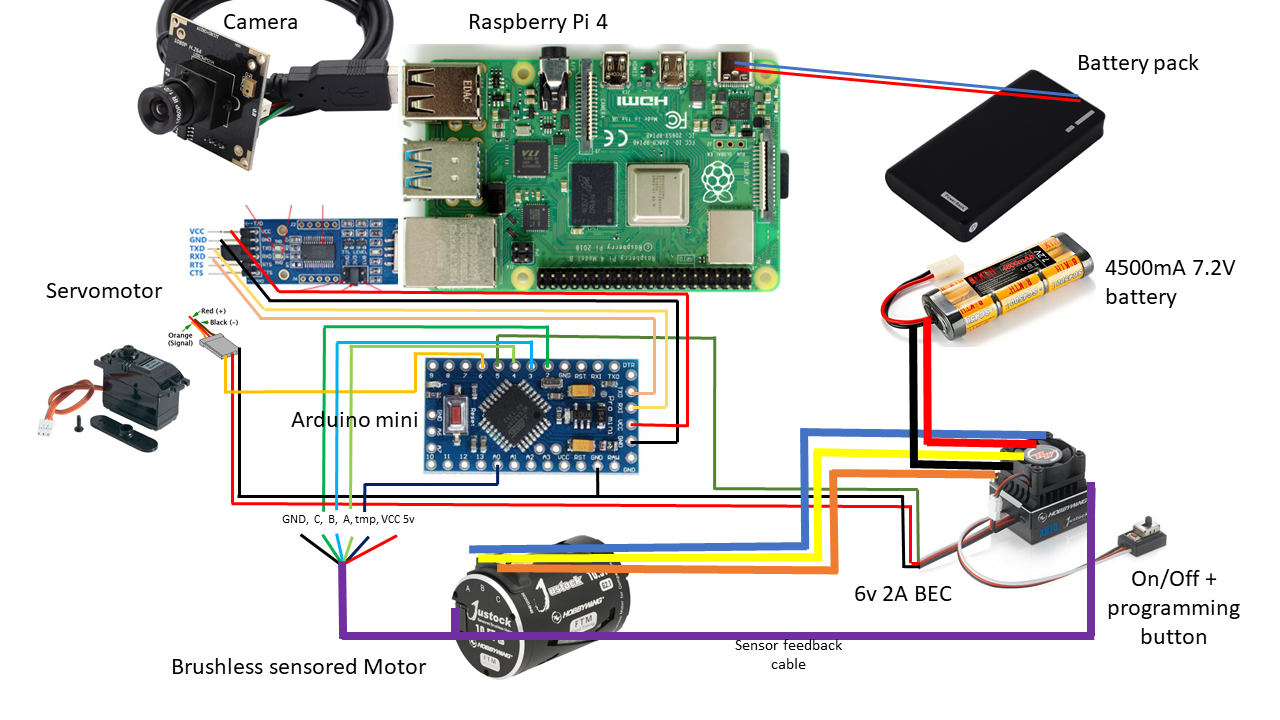
\includegraphics[width=27cm]{../../docs/schema.png}}


\subsection{Software}
As you understood, our work will be focused more on the software side.
Our project will be written mostly in Python, with a bit of Java Script(JS) and arduino code.
We will divide the project into 3 big parts:
\begin{itemize}
\item The backend. This is where most of our efforts will be focused; this part includes every key program all the way from the data gathering to the model training and testing.

The first part we will develop is the code responsible for the communication between the RaspberryPi and the Arduino, this code will enable us to drive the motor and servo motor by calling some simple functions. This program will also later be used to fetch the speed of the car transmitted by the Arduino to the RaspberryPi.
Then, we will need to find a way to control the car manually, for example using a controller. The values of every axis and buttons on the controller will need to be fetch and then transmitted to the arduino using the code previously created.
We will then create functions to capture, save and load images and annotations corresponding to the image. The data will be stored in an ordered manner using the date of capture of the images. For this part we will mostly use OpenCV and Numpy.
Then we will need to create models using Tensorflow, we will firstly create a basic Convolutional model. In order to train it, we will need to write a program to load existing data, feed the right inputs and output to the model. The modularity of this part is crucial as our models will have more and more inputs and outputs.
To increase the accuracy and generalization of our model, we will need to provide some augmented data to our model. We will create multiple functions to add some random noise, random shadows, lights, and blur to our images. This process known as data augmentation, is really important and will bring more robustness to our models.
We will then be able to start our optional objectives such as speed control!

\item The Telemetry website.

Developing an autonomous car is difficult. The more you know about what’s happening inside, the better results will get. We will use telemetry. It will help us analyze what is happening inside the car at any moment. To collect data, a server will run outside the car on a computer. The car will communicate with the server through a Wi-Fi router. The server is divided in two parts: The first part is a web-app. It will use JavaScript (Node.js) as the main language. The UI will be created using the React.js framework. The server will handle image streaming with UDP from multiple client (autonomous cars). The web-app will display the camera’s views in a canvas. All the logs will be accessible from the web-app and will be displayed in various forms as Time series graph and Scatterplots. The server and the database will run each inside its own docker container. We will use docker-compose to run all containers with one command.

\item The presentation website. The presentation website will be a Static Generated Site built with Next.js (a React Framework). The Website will introduce a cool design, a presentation of the members and the progress of the project. It will be hosted on GitHub Pages as it is free, reliable and can be managed on the same organization account.
\end{itemize}

\newpage
\subsection{Constraints}
Throughout the project, we will have to keep in mind some constraints.
Our biggest constraint will be the compute power. We need all of the inference of the model to be executed on the RaspberryPi, this means that we will have to be really careful of the performance of our code. How fast our main control loop is will determine the reactivity of our car. Our usb camera can capture up to 30 images per second, our main control loop should ideally match 30 iterations per seconds. For example, if the car is going at 1 meter per second and our control loop is running at 10hz, the distance the car travels between each iteration is 10cm. Now if you are going five times faster with the same control loop, you now have 50cm between each decision, this is huge for such a small car! The part that will likely take the most time will be the inference, we will need to keep track of the ratio between performance and accuracy of our models.
Regarding the accuracy of our models, we will need sufficient accuracy and generalization to be able to complete multiple laps. If the generalization is not high enough, small changes in the lightning or changes in the background will affect the prediction of our model.
On the safety part, we have to keep in mind that we are driving a powerful car, a wrong motor command can lead us right into the wall and break the car. Prior to deploy and test our code on a real track, we will need to carefully test our code to avoid such a disaster.

\newpage
\section{Realized tasks}

\subsection{Project Setup}
Before starting to program, we had to set up a good GitHub repository. First, we created a new GitHub Organization called Autonomobile, this is where all of our repositories are located. We then created the AutoPylot repository. We decided to put everything related to this project in the same repo for simplicity, so we have a repo divided into four main parts:
\begin{itemize}
\item The autopylot python module. While creating it, we searched online for best practices regarding python packages. We learned a lot regarding that part ! We put in place a python virtual env (venv) so that every member could easily install every required package: OpenCV, Tensorflow, NumPy and more.
\item Some main scripts that use autopylot module.
\item Everything related to the presentation website and telemetry website.
\item Documentation! Even if it is not the funniest part of the project, it is still a really important one: keeping track of how to install the project, our dependencies and so on. We also keep in this part every project report and work we had to do for the presentations as we may need them in the future! It is important to keep track of what is done and what is to be done!
\end{itemize}
We also created a GitHub action to automate the testing of our project! Every important function coded is accompanied by its set of tests. This enables us to assert that the code we are currently working on works as expected. With this idea in mind, we added a really important rule: no addition of code on the main branch if it doesn't pass all the tests we wrote. This rule is really important to keep main clean from any major bug! This rule induces one thing: we need to open branches and do Pull Requests for every feature we add to the project. Moreover, we need the approval of someone else to merge the Pull Request into the main branch. We all forced ourself to respect this as much as we could, the result is that now we are totally used to this process and everyone is aware of what people are working on because they need to review their code.
On top of that, before committing code, we run a code linter that clean our code, adds and removes whitespace where they should or should not be, rearrange long lines so that they fit into the screen. \\
All in  all, we are confident to say that we came up with a great set of rules and a great project structure to avoid spending time on solving issues that could arise from a poor project setup.

\newpage

% Ellerbach
\subsection{Arduino and car control}

\begin{figure}[b!]
    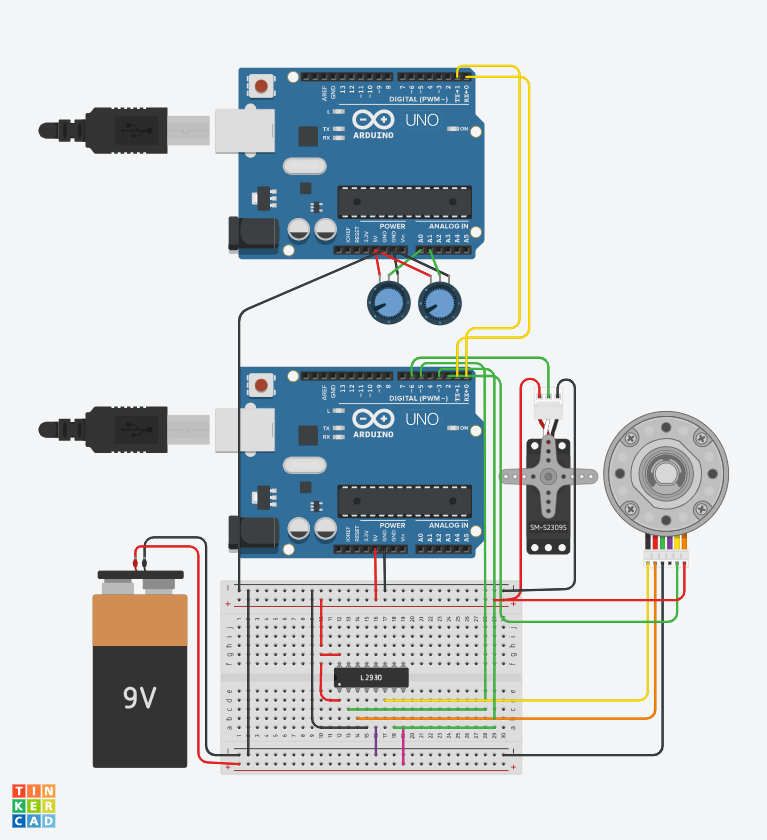
\includegraphics[width=\textwidth]{../../docs/car-hardware.png}
    \caption{TinkerCad Circuit}
    \label{fig:tinkercad}
\end{figure}

This task is essential to the success of this project. This is the lowest code level we will deal with. The Arduino code is the code that drives our motor and servomotor, without this part nothing works! Any issue coming from this part of the code would mean a crash into a wall. To ensure that this part was working as expected, we run a lot of testing with the real car, trying different scenario to see what to expect for example if we lost the connection between the Arduino and Raspberry Pi or if it did not receive orders for a given amount of time. As all the team could not have direct access to the car, we did a virtual clone of the car using TinkerCad, simulating and live debugging our code before feeding it to our real car!\\
You can see on the figure ~\ref{fig:tinkercad} the TinkerCad simplified version of the car.



You can see here two Arduinos, but on the car we only have one, why is that? TinkerCad did not have a Raspberry Pi, so we added another Arduino to simulate the serial connection between the Raspberry Pi and the Arduino. The Arduino on the top sends steering and throttle information (as the Raspberry Pi would do) to the other Arduino that processes this information received on the serial port and then controls both the servomotor and motor. They are both running on a 9V battery here but in real life on a 7.2V battery. We then read the signal sent by the sensored motor, using an interrupt pin. The rpm of the motor is then deduced from this signal and then sent back to the Raspberry Pi.
This virtual simplified car really helped us in the process of developing the core of our car!

When the Arduino part was finished, we could start the python part, that consisted in sending the right bytes to the serial port connected to the Arduino, it was hard to debug when there were issues on the one hand, but really satisfying when it did work! We are now able to send steering and throttle to the Arduino making the car controllable using python!

% Ellerbach
\subsection{Camera}
The next step was to build a class to fetch images from our webcam, thankfully, the python module OpenCV has already some functions to do exactly that! \\
We only needed to add a wrapper around all of that to match our needs. We are now able to fetch images from our camera into a NumPy array that we can manipulate. On top of that, we did create a `dummy` version of this camera class in case we did not have access to a camera to run some tests, this class return a black image when we grab a new image form it. We use this class in some of our automated tests.

\newpage 

% Girold
\subsection{Load and save data}
In this section, we will talk about how we can load and save data, data is defined as an image.png or the same image as a JSON file. We want to have both types of data because the JSON files are easy to manipulate and the png images will be used to display the images captured by the car's camera.\\

Let’s dive deeper into how we managed to make it work. Firstly, we will need to make use of different modules and packages. For this part, we will use three modules: Json, cv2, and os. A more detail explanation of those modules can be found in the next section.\\ 

 
Let’s go throw the different functions: \\ 

Firstly, we have the load functions. There are present to make it easier for us to use images for future functions. The first of these functions load’s an image (.png) from a given path and returns it as a NumPy array (multidimensional array object) which is amazingly fast for computing a large amount of data, exactly what will we do in the future.\\ 

Secondly, we have the function save. These are simple but are quite important. Indeed, the first save function simply saves an image given as a NumPy array to a file. The second one saves a JSON file into dictionaries of the content of a JSON file. 

One important function which will be used later is the save image data. 

The goal of this function is to save an image as a NumPy array into two files, one .png and the other one .json. We will use this function quite often throughout the next weeks.\\ 

As for all the functions we will make, we will want to make sure they are working correctly and the way we intended them to. To do so, we must make test functions. Writing tests is essential to be able to maintain clean and usable code. It certainly is necessary for preventing problems with your code later. It will also help when adding new functionality or refactoring your code, making sure you haven’t broken anything you didn’t intend to. This is done through the use of assert and yield which have different properties which we will not discuss here as they aren’t the main subject of our project.\\ 

In this case, we will make use of four different modules: os, shutil, NumPy, and test. To successfully conduct the tests, we need to create a temporary directory, we will inside this directory then remove it at the end.  

The test to the load and save function have 10 function which tests each function on specific outcomes. We want to be sure that our functions do save the images and JSON files into the correct directory.  

\newpage 

% Gay
\subsection{Data set}
Previously, we created functions to load and save data, those functions handle JSON files and images. \\ 
Now we have to deal with data set but first, what is a data set? \\  
A data set is a folder which contains JSON files and images. Each file will have in its name the date followed by .png, the JSON should have the same name, but it ends with .json instead of .png. In order to have the date, we have to use the time method time() which returns the time as a floating-point number expressed in seconds since the epoch, in UTC.\\ 
Why are datasets so important? \\  
The goal of these parts is to manipulate data set. We take the information that the camera is giving to us, and we can load, save and sort those data in a cleaner way so that our training model and our Artificial intelligence model can use it.\\ 
We started by creating two files, the dataset.py file for the main functions and the test dataset.py in order to provide test functions to see if our code is working.\\ 
Firstly, for the dataset.py file, we had to import two modules. \\ 
The first one is the glob module which finds all the path-names matching a specified pattern according to the rules used by the Unix shell.\\
The second one is the os module. It provides functions for interacting with the operating system.\\ 
Secondly for the test file in addition to the module glob and OS, we used the sys module. It provides access to some variables used or maintained by the interpreter and to functions that interact strongly with the interpreter. 
We also used the shutil module which offers a number of high-level operations on files and collections of files. In particular, functions are provided which support file copying and removal. Furthermore, we used the NumPy module to deal with matrices.\\ 
The dataset file is composed of ten functions:\\  
The first is the load dataset function which load JSON and PNG file from a folder, the function takes the path of a directory which contains JSON and PNG and it returns a list of dictionary containing the image and the JSON file.\\ 
The second function is the load multiple dataset, it is similar to the load dataset function but deals with multiple images and JSON files and it returns a list of lists of dictionaries.  We also had a second argument named flat, if flat is equal to false, it means that we have to deal with a list of lists, otherwise we have to deal with a simple list.\\ 
The third one is the load dataset generator function, it iterates image data, generators do not store all the values in memory, they generate the values on the fly.\\ 
The fourth one is the load multiple dataset generator. It is similar to the load dataset generator, but it deals with several images and JSON files.\\ 
Then the load sorted dataset function sorts the loaded data and returns a list of dictionary containing sorted data. Thanks to the function time.time() we have a chronological view of our elements, and we have to sort them. We had to use 2 subfunctions, the first is sort paths which sort all our elements thanks to the sorted function and the second subfunction is the get time stamp. The function split the name of an element in order to have only the part containing the date without the .json or .png and then it converts it into a float.\\ 
The load multiple sorted dataset is similar to the load sorted dataset function but it deals with multiple dataset and returns a list of lists of dictionaries.\\ 
The two last functions are the load sorted dataset generator and the load multiple sorted dataset generator.\\ 
It iterates sorted image data and do not store the values in the memory.\\ 
The test dataset file is composed of twenty-one functions.\\ 
We started to create the convert path function which is useful to convert paths according to the current OS because we encounter a major issue when we ran for the first time our test. Indeed, some errors appeared under Linux while under windows everything works because the loading order is different under linux than under windows.\\ \\ 
Then we created the test sort paths is sorted function which test if the function sortpaths returns sorted elements. \\ 
The third function is the test get time stamp. It tests if the get time stamp function works, and if the value that it returns is a float. \\ 
Afterwards, we had to create a test directory to generate files containing image datas with an image, some datas like the steering and the throttle in order to test the other functions. \\ 
Firstly, we check if the number of files that we have created is the same number present in the test directory. \\ 
Secondly, we check if the load dataset function was working using the previous files that we have created. We did the same test for the function load dataset generator. \\ 
Thirdly, we have to test if our functions are capable to sort our dataset, by naming our files with different dates we can check if after the function load sorted dataset we have a list of dictionaries in increasing order. \\ 
Afterwards, we created multiple directories and multiple files to test our function that take as parameters multiple directories. \\ 
We have types of function load multiple dataset, with have a flat version and a not flat version. \\ 
The difference is that for the flat version, datas are in the same folder and for the not flat version, datas are in different files. Our test is successful as we can collect our files independently of their folder. \\ 
We made the same test for the function test load multiple dataset generator not flat and for test load multiple dataset generator flat. \\ 
To finish, to get a cleaner workspace, we delete all our folders created for those tests. \\ 

\newpage

% Ellerbach
\subsection{Data visualization}
In order to properly visualize our fetched data, we created some utils functions to do so.
The figures ~\ref{fig:a} shows a left turn and ~\ref{fig:b} a straight line. \\ But How does that work ? \\ Each saved images have labels: steering, throttle and speed, once we load them using our previously developed functions, we are left with a dictionary containing the image in a NumPy array, and floating points values steering, throttle and speed. We then draw onto the image some lines and text using OpenCV's functions. We draw a line in the middle using our steering float, the line on the right represents the throttle, and finally on the left, the speed! We designed those functions to be as modular as possible, if we ever need to add a new data to visualize, we just need to add a single line! You can imagine layering outputs of different models to determine which one is better. We can also imagine in a near future that our model would predict positions with confidence metrics, we could totally represent those using those visualization functions. In short, they will be essential to debug what is going on and provide key information to our eyes.

\begin{figure}[h]
    \centering
    \subfloat[Left Turn]{%
        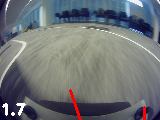
\includegraphics[width=0.49\textwidth]{../../docs/left-turn.png}%
        \label{fig:a}%
        }%
    \hfill%
    \subfloat[Forward]{%
        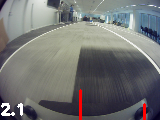
\includegraphics[width=0.49\textwidth]{../../docs/forward.png}%
        \label{fig:b}%
        }%
    \caption{An example of two visualized images}
\end{figure}

\newpage

% Bobovitch
\subsection{Basic car loop}
This is a mandatory part. It contains the main function to run. The Main Control Loop will call various processing functions. We successfully achieved fetching of images from the camera, fetching commands from the controller and we successfully updated the general car memory state so now we are able to send multiple signals and commands to the hardware driver. \\

We made real life testing that confirmed our progression. We plan next to maintain our modular philosophy to easily add or remove features. This part seems easy to implement but remains one of the most important. We have to be sure that each component and modules are working perfectly to avoid performance issues. \\

Now we will mainly focus on the driving part and the neural network.

\begin{figure}[h!]
    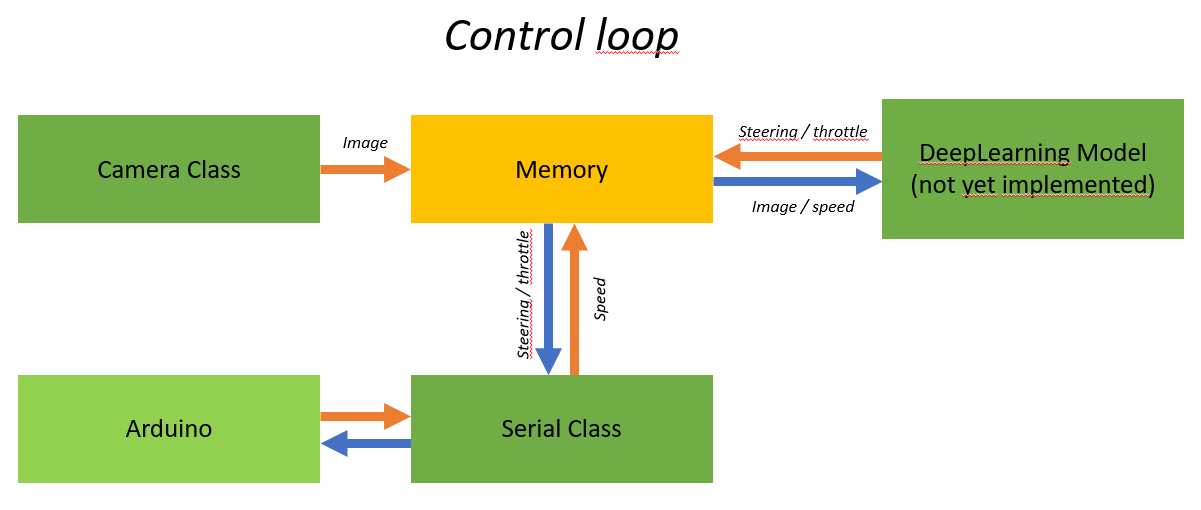
\includegraphics[width=\textwidth]{../../docs/control-loop.png}
    \caption{Diagram of the Control loop}
    \label{fig:control-loop}
\end{figure}

% Ellerbach
\subsection{Logging}
While executing for the first time our driving script on the car, we thought that our current way of logging and keeping track of events could be drastically improved. To answer this need, we came up with an idea: have the logs sent to the telemetry server. This could enable us to directly have access to what is going on in the car in real-time! On top of that, we would also have the logs stored locally in a file on the Raspberry Pi and printed on the standard output. \\  

So we began searching for a nice way to do this easily without having to change our project's structure. The idea is to be able to send both logs and telemetry with the same process, but the telemetry should not be saved to file and only sent to the server. We found the python module `logging`, that comes with python without further need of installation. Logging enables flexible event logging for both modules and main scripts. After trying up some example scripts, we decided to go with this module! In a first time, we added and set up the file handler and stream handler that respectively logs to a file and to a stream (in our case the standard output), those two handlers listens only for logs and not telemetry. Then, we had to develop a handler that would fit our needs to send both logs and telemetry to the telemetry server, we found a socket handler that somewhat fitted some of our needs, but not all. So we started a custom handler with having in mind this socket handler example. \\

This handler development is parallel to the server's development. This requires an efficient communication between the team developing the logging (client) and the one developing the server. This part will be executed on the Raspberry Pi, so it has to be light to avoid overloading the CPU, also we have to keep in mind that the network might be limited so in a case of a telemetry log (sending an image), the image has to be compressed in real-time, again while finding a performance balance.
We came up with a prototype of the python client with a simple python server, but have not completely finished the telemetry server. When the handler is called with a new log to send, it is being added to a queue of logs and telemetry messages, those are being sent by a thread so that we do not wait for the item to be sent to continue in the program. \\
To conclude, this part will be of great help for debugging and will be allowing us to go back in time after a run and take a look back at the main events we had, crashes and more. We aim to have this part finished and functional by the next presentation.

\begin{figure}[h!]
    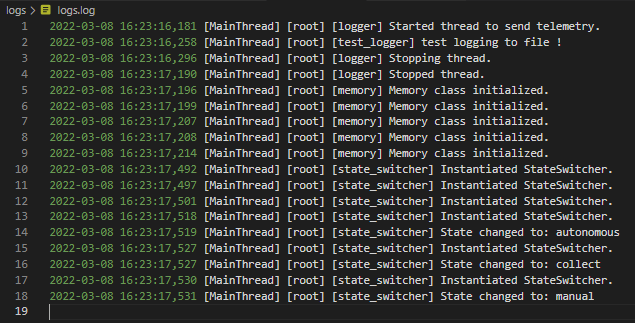
\includegraphics[width=\textwidth]{../../docs/logs.png}
    \caption{Preview of the logs saved to file}
    \label{fig:logs}
\end{figure}

\newpage 

% Bobovitch
\subsection{Telemetry}
Why use telemetry? \\

In our context, we face different problems that may be hard to solve without accessing the device. Our code runs on an Rasberry Pi which make difficult the debugging.\\

Moreover, artificial intelligence is a black box. We don't know what's happening during the execution process. That said, once the program has finished, you can observe the past events thanks to the logs. However, this approach to debugging is not practical and not efficient enough for our use case. To better understand the background processes, we decided to use telemetry. It will allow us to collect valuable data in real time.\\ 

Since we are dealing with an “intelligent” device, we should fully control it at any moment. It would be a disaster if the device does not obey us, as it can create a security treat for the environment. As we know, security is always one of the most important point to keep in mind. In the case where the car is moving at full speed towards a child, how could we stop it?\\

We came to the point of building a telemetry server combined with a remote controller. It will fill all our requirements. Especially it will offer us a great balance between security, ease of use and functionality.\\

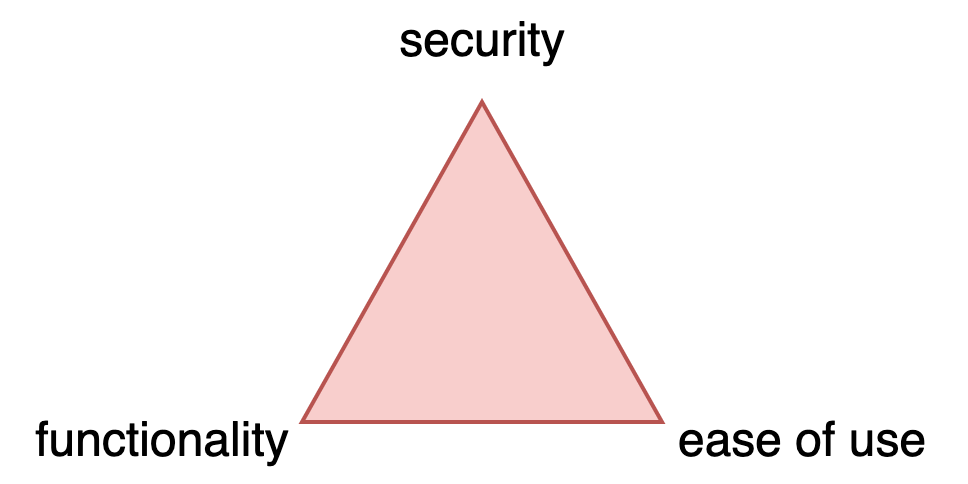
\includegraphics[width=\textwidth]{../../docs/diagram2.png}

\newpage

We will benefit from great portability, an awesome development process, and a powerful UI. The server makes it possible for us to communicate with the car in real-time. We can detect any problems before they happen. We can control the car without any limitations. We can remotely stop and restart. We can remotely update settings. And we can remotely view logs and car updates.\\ 
Now let's see how we implemented this. As seen previously, we have already set up a logger which records the information continuously. Firstly, we extended the functionalities of the logger while maintaining a modular philosophy. The logger gained the ability to send logs and images through a Wi-Fi network. Next, we were confronted to a different challenge: How to send a decent amount of information to multiple clients of different types (web-browsers and raspberry pi hardware) in real-time?  We choose to use Socket.io . This an excellent open source cross-platform library. Socket.io enable us to create bidirectional and low-latency communication. 

Here is a simple exemple of a communication between a client and a server in javascript. This simple API, simplifies our development process and make data transmition more compliant.\\

\centerline{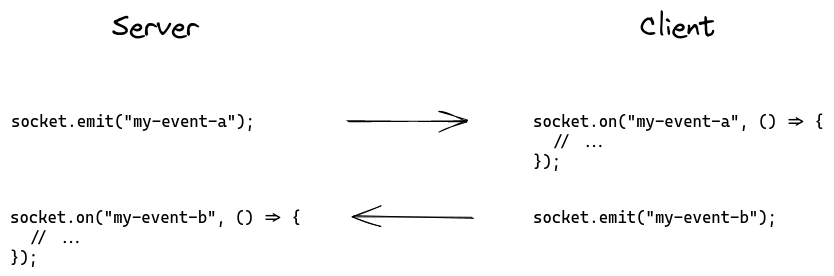
\includegraphics[height=5cm]{../../docs/server-client.png}}

But “[Scoket.io](http://scoket.io/)” does not stop here. This library is much more powerful. We have the possibility to broadcast a message from the server to all clients:\\ 

\centerline{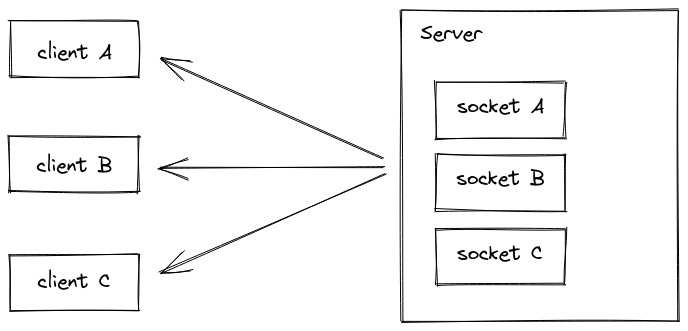
\includegraphics[height=6cm]{../../docs/broadcast-0.png}}

We can even broadcast from a client to other clients:\\

\centerline{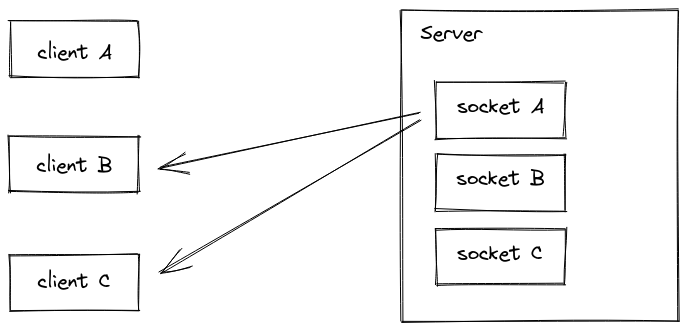
\includegraphics[height=6cm]{../../docs/broadcast-1.png}}

We can even go further by using the concepts of rooms. This means that each client can join a sort of group chart where the server can easily target this group chat:\\


\centerline{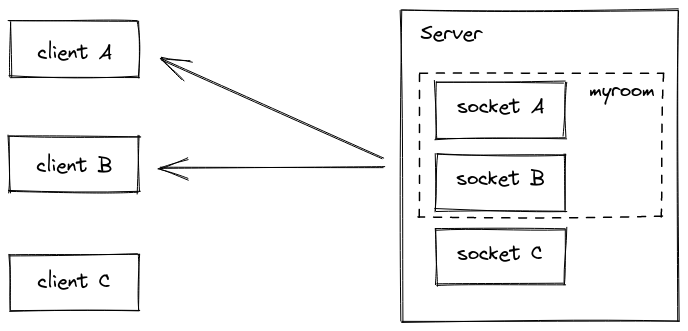
\includegraphics[height=6cm]{../../docs/rooms.png}}

From now, ui-clients|web-clients|people mean a socket.io client instance which runs in a web-browser. A car|py-clients is a socket.io client instance wich runs on a raspberry pi4.\\ 
As our main goal is to win races, which implies multiple cars on the track, we have to thinks about a way to manage multiples cars at once. At the same time we wanted every clients of the network would be able to communicate with each other (web-clients with python-clients only). Our design choice was to implement a TV-like mechanism : a web-client can only stream one py-client. And a py-client can send content to an unlimited amount of web-clients, meanwhile a web-clients has the possibility to switch cars at any time.\\ 

\newpage 

Socket.io is just a tool. We developed a high performance server wich is acting as a middleman between clients:\\

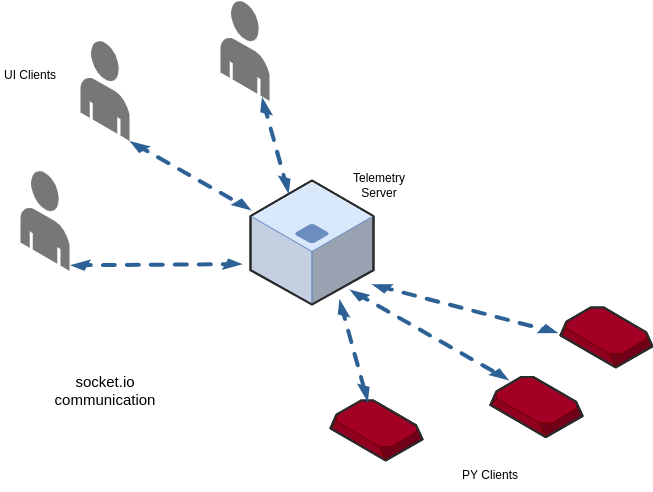
\includegraphics[width=\textwidth]{../../docs/diagram.png}

The server uses the JavaScript language (Node JS) as it offers great flexibility, it is very efficient for networking and IO tasks thanks to its language design. Nevertheless, it requires great vigilance because the language is not typed. Any bug could lead to performance issues and memory leaks. But it still remains the best choice for us. We made a great test coverage to extract all bugs.\\ 

The server is battery included, which means it comes with an exeptional UI inspired by the familiar material design by Google. The web-app is intuitive and feel right at hime. To build the UI we used the “Next.js” framework which is server side rendered react with an API endpoint. “Next.js” is a top-level industry react framework used in many compagnies.\\

\newpage  
Here was the first prototype:\\ 
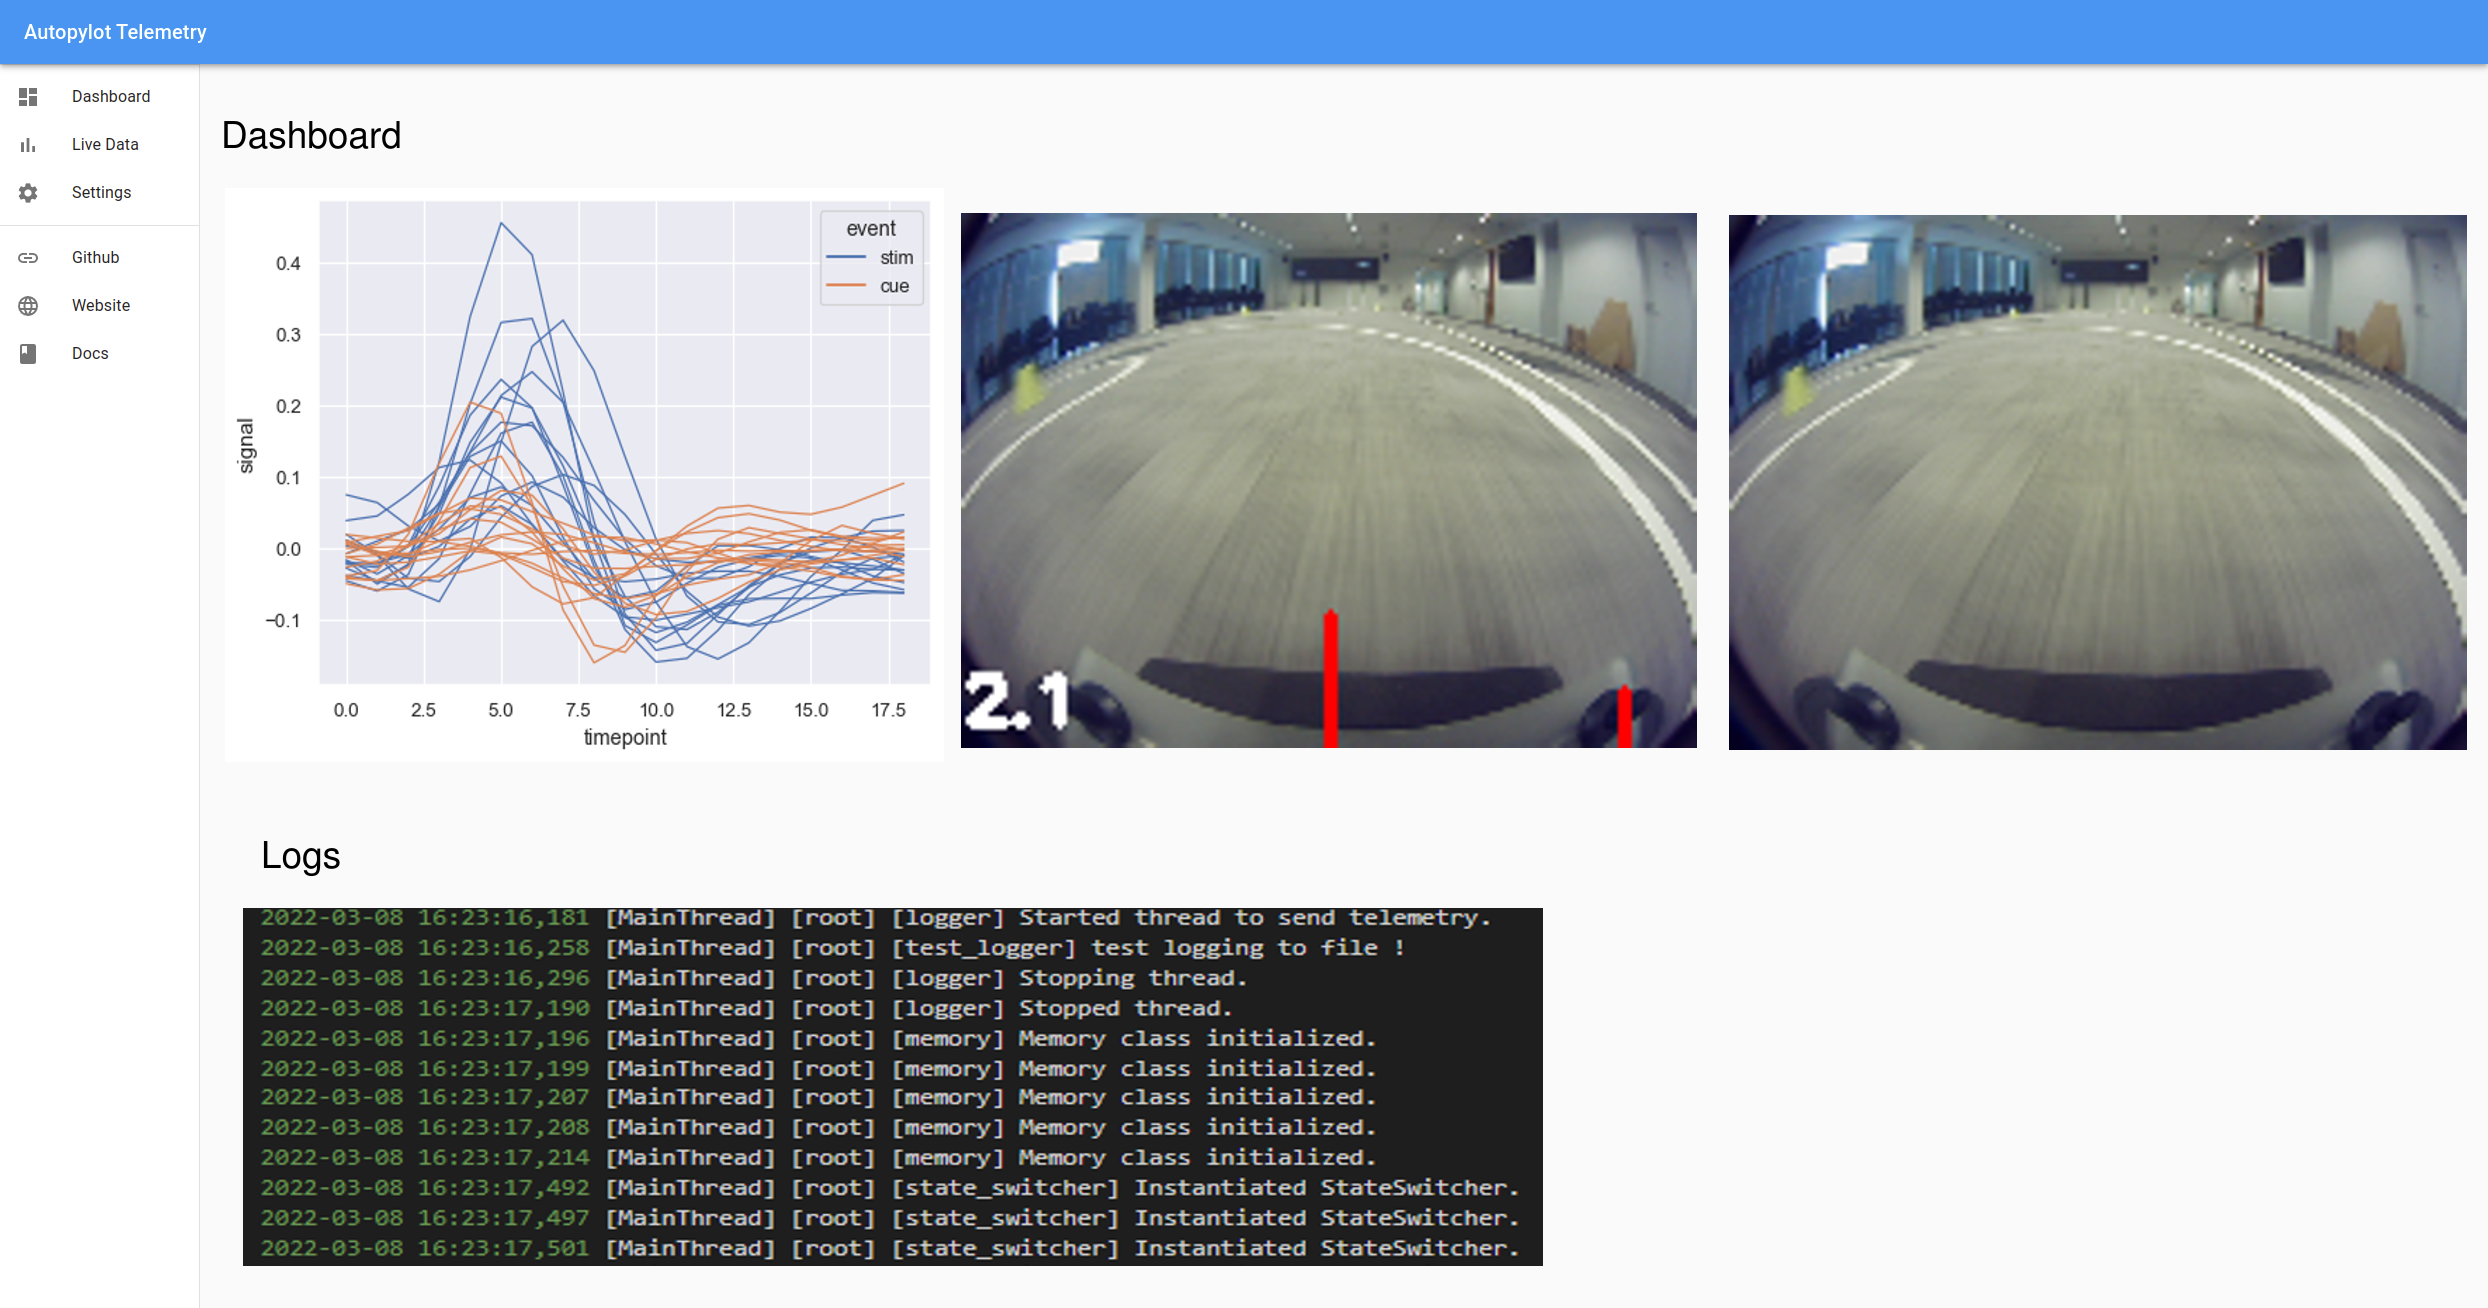
\includegraphics[width=\textwidth]{../../docs/telemetry.png}

Here is what we have done:\\
\includegraphics[width=\textwidth]{../../docs/Telem1.png}\\

This is the “Main Dashboard”. This section contains many information about the car. For instance by looking at the steering chart, we observed that in straight lines our car behaves very calm and predictive. And during a turn we have smooth curves which indicate us that we are on the good path. We also have the trottle and speed charts and even the CPU and RAM indicator. This very nice to have it because we are working with embedded systems and ressourses are limited.\\
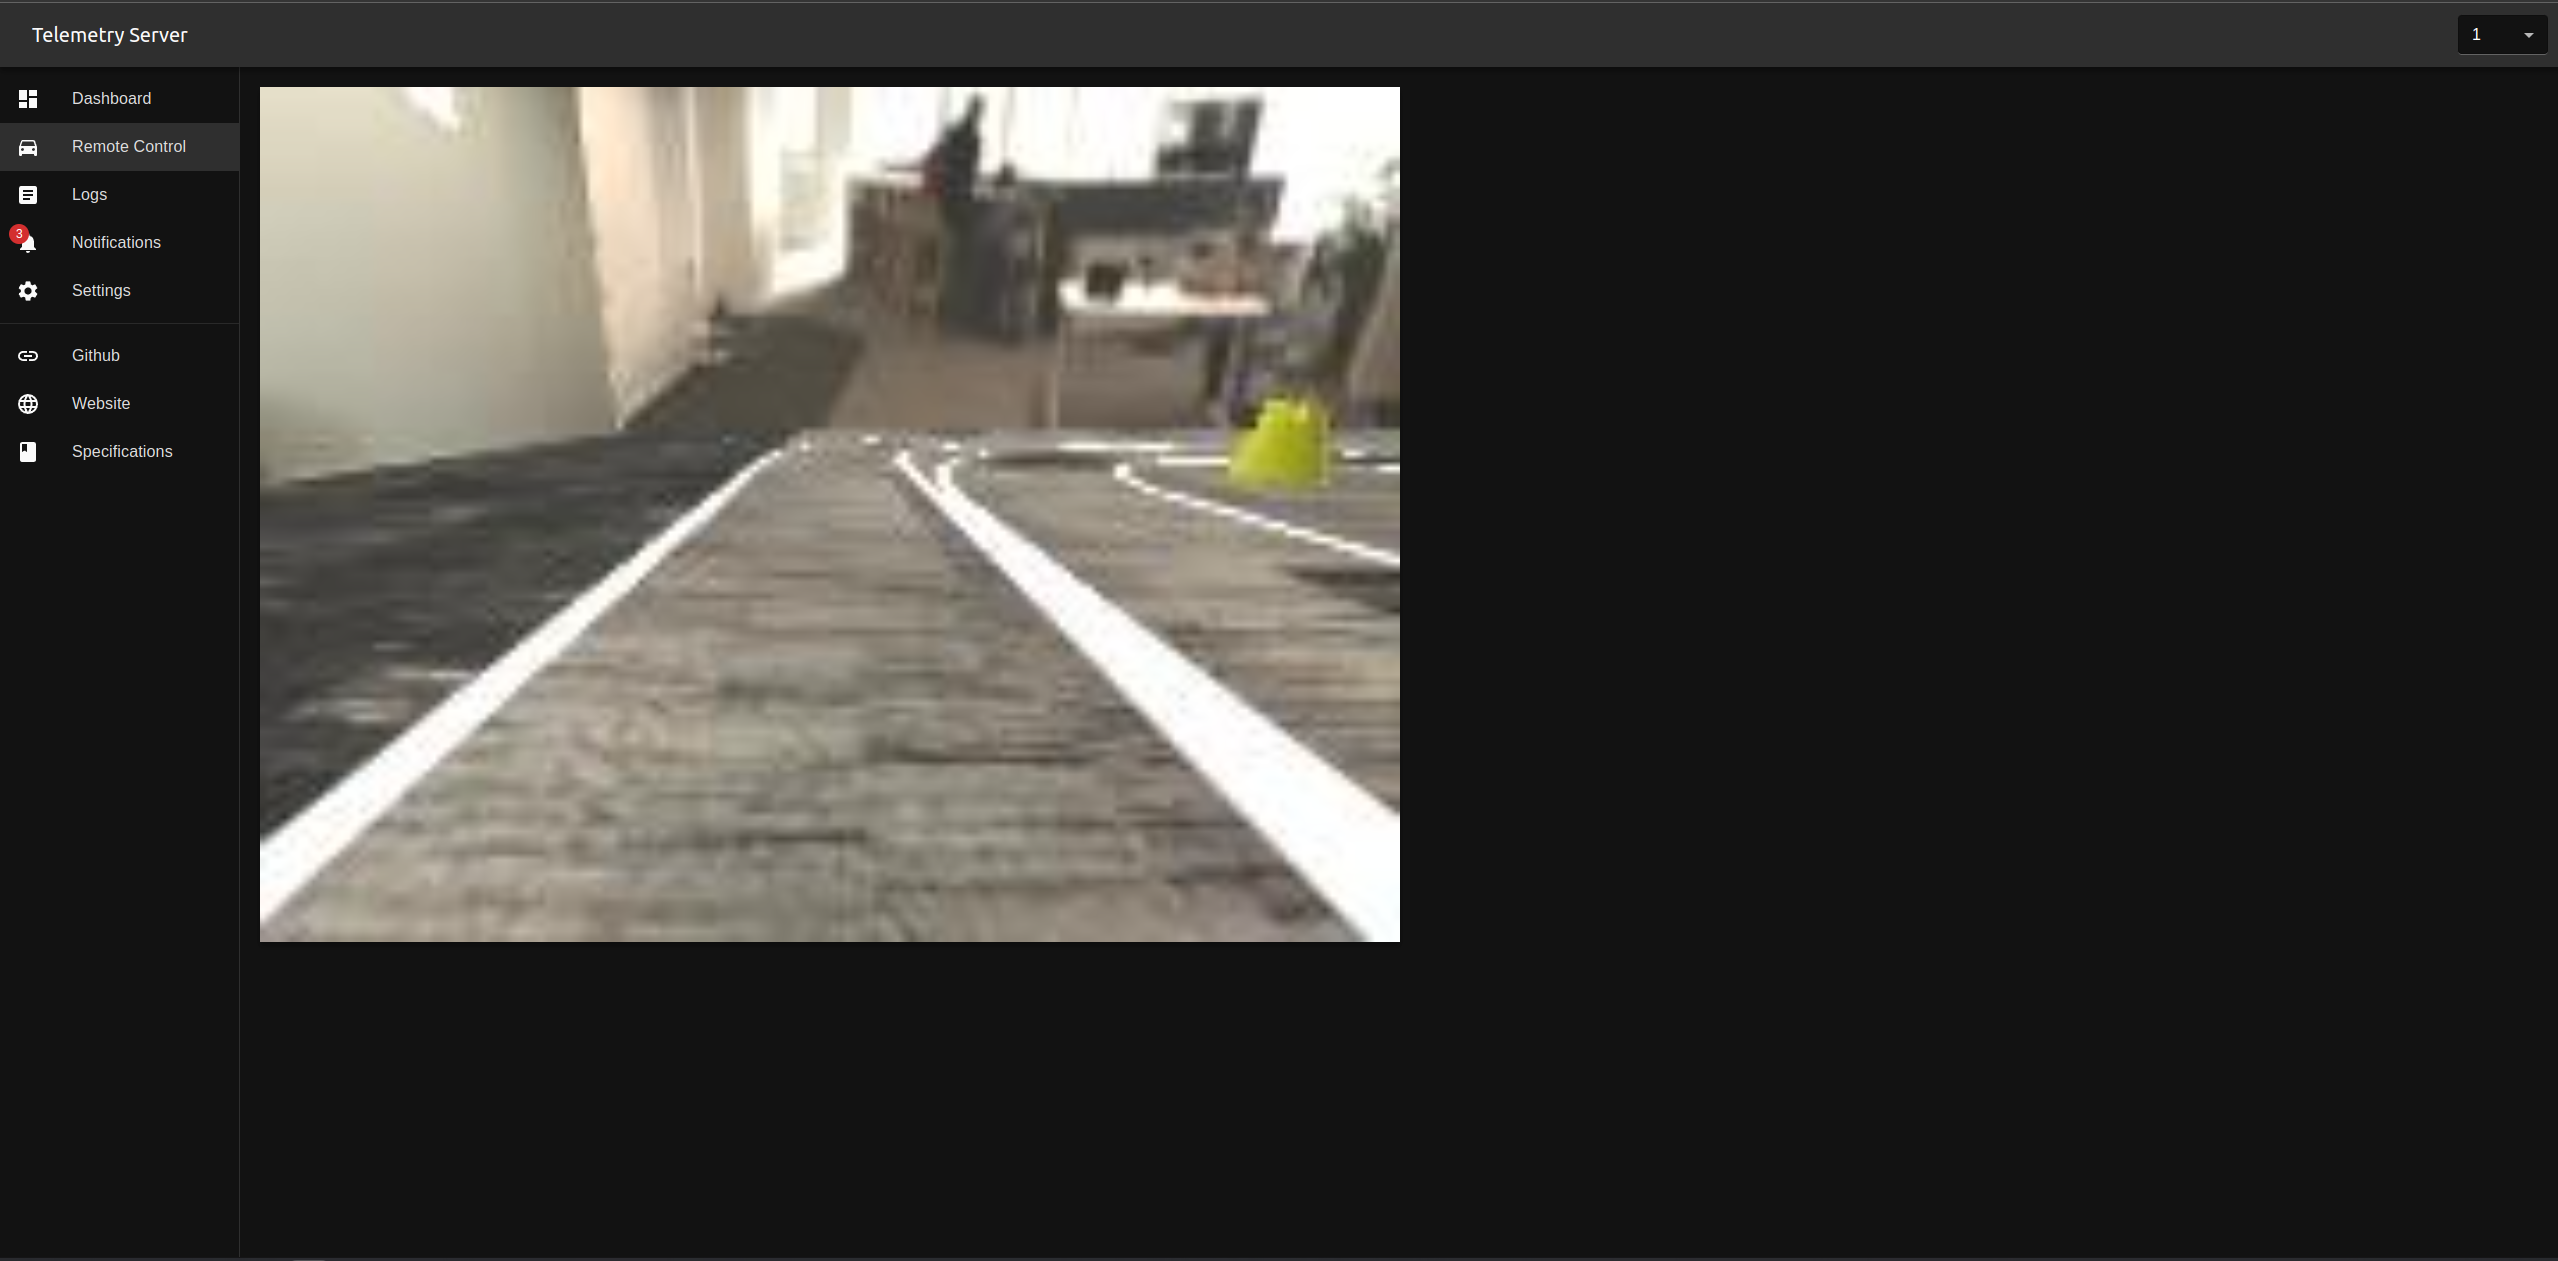
\includegraphics[width=\textwidth]{../../docs/Telem2.png}\\

This is the “Remote Control”. This section help us see that the car actualy see in real time. Nothing to say more expted that it’s very cool. We use this in training to we can actualy see better when we drive. When the car is in autonomous mode we have a nice FPV which help us understand where the car is making it’s decision.\\
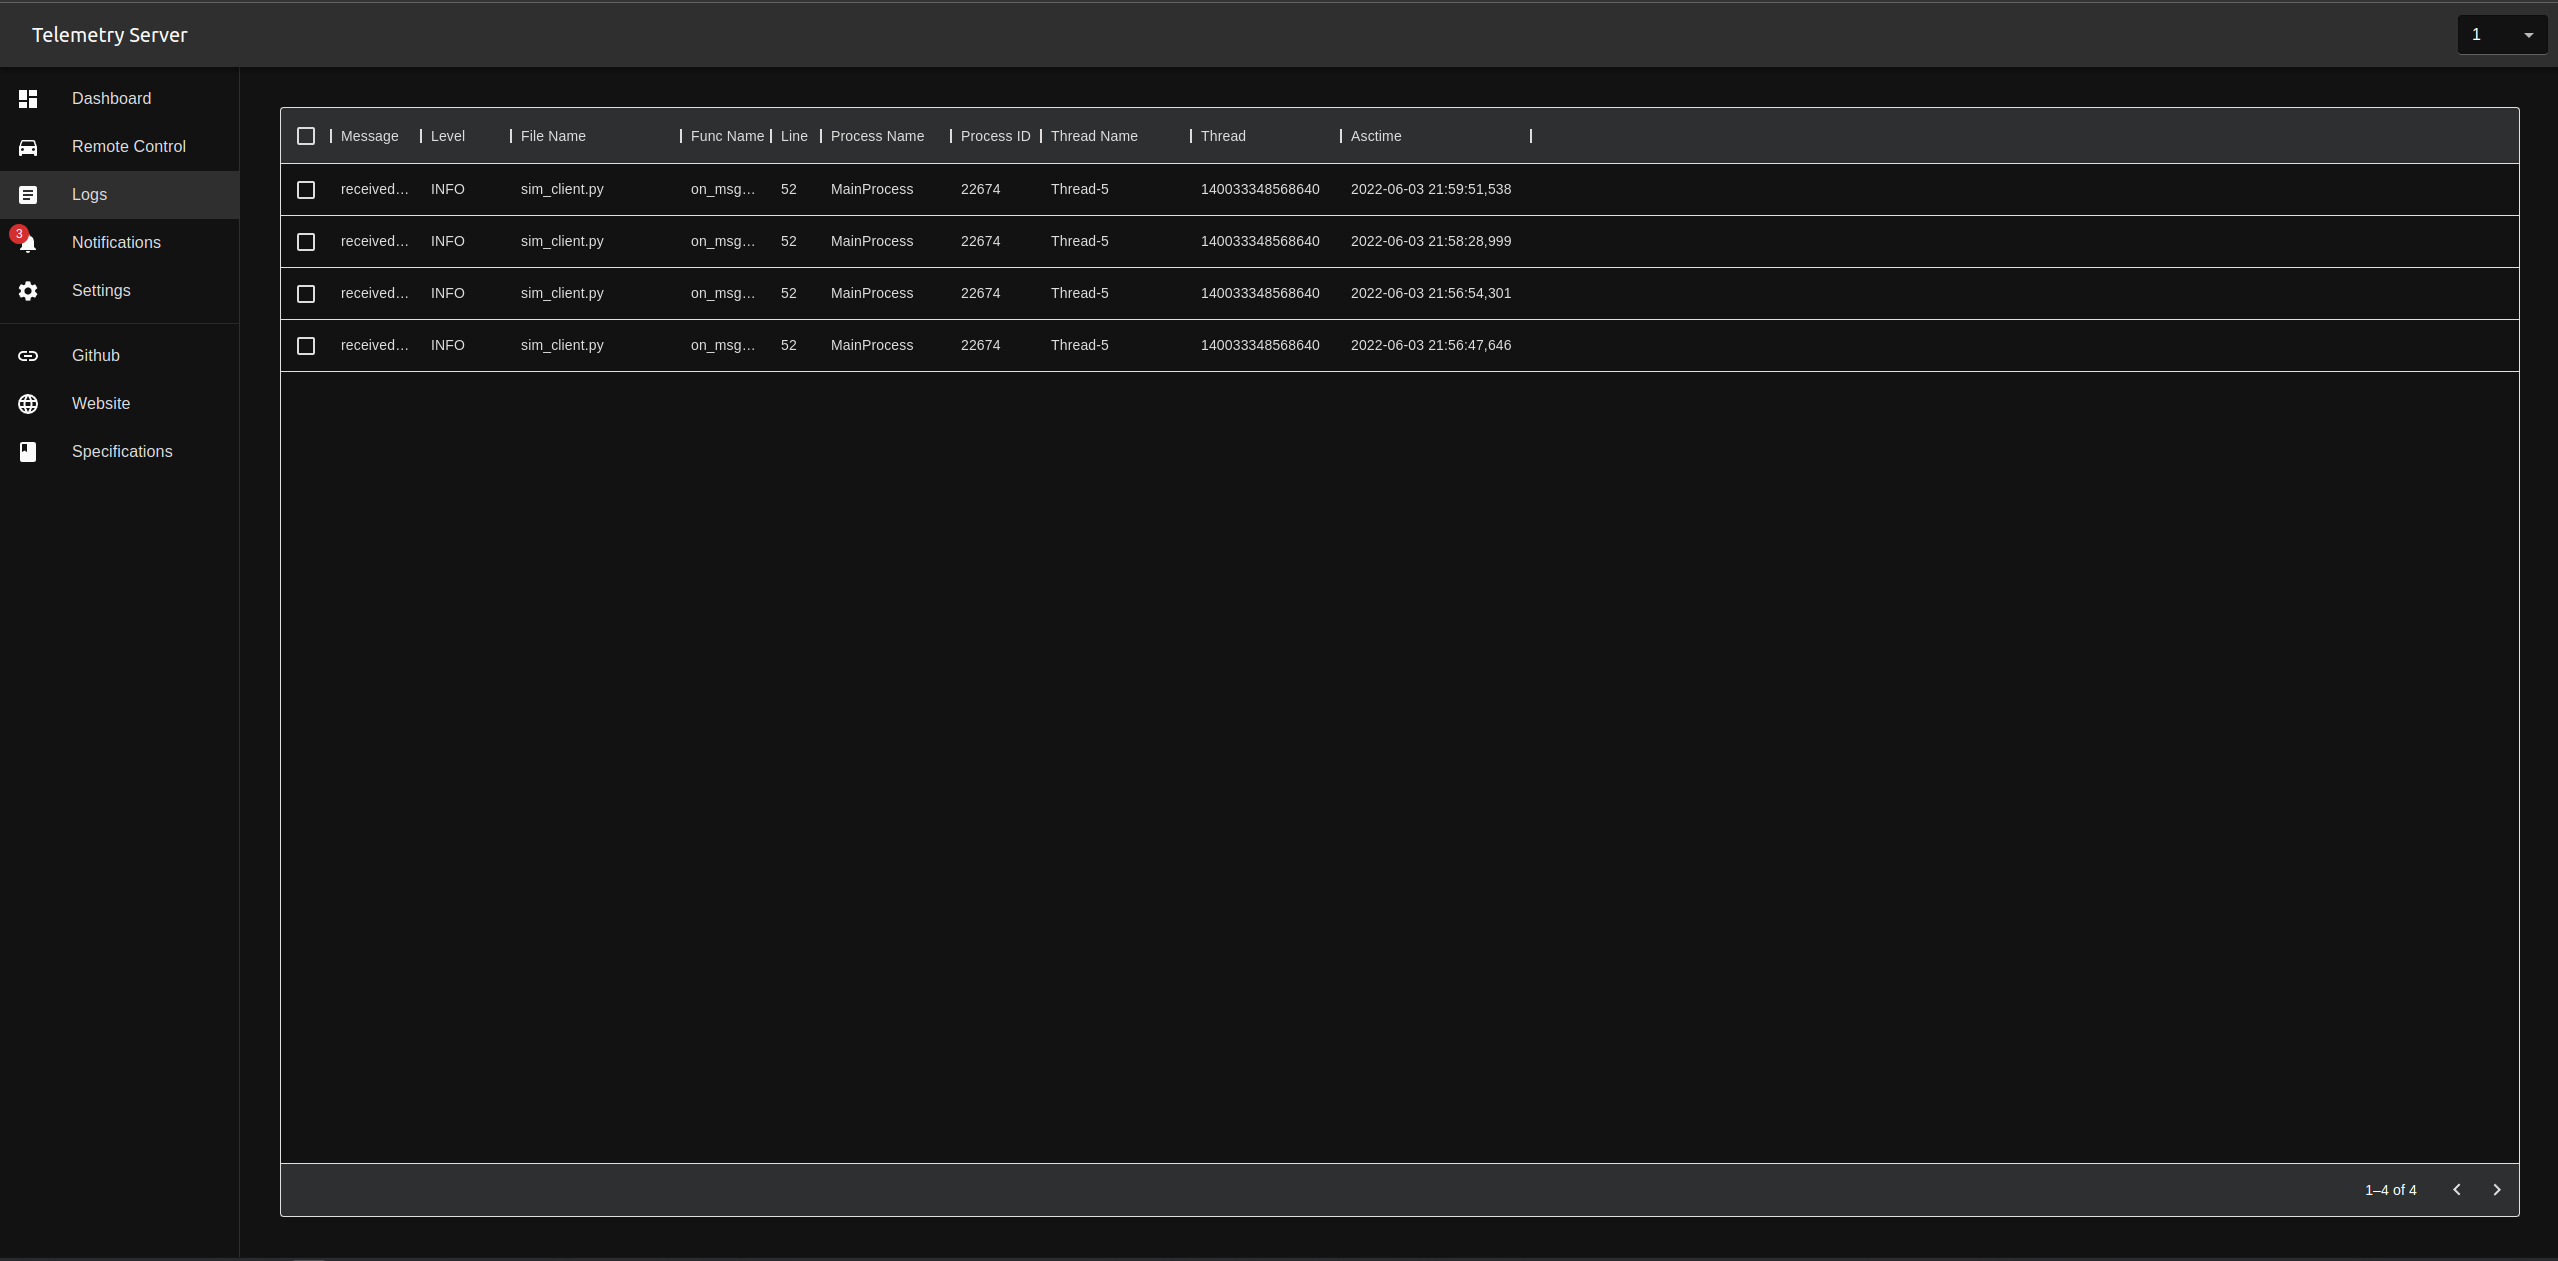
\includegraphics[width=\textwidth]{../../docs/Telem3.png}\\

Here are the “Logs”. When someting happen, a new row is inserted. This table support searching. When we have thousands of thousands of logs we can quickly find any message.\\
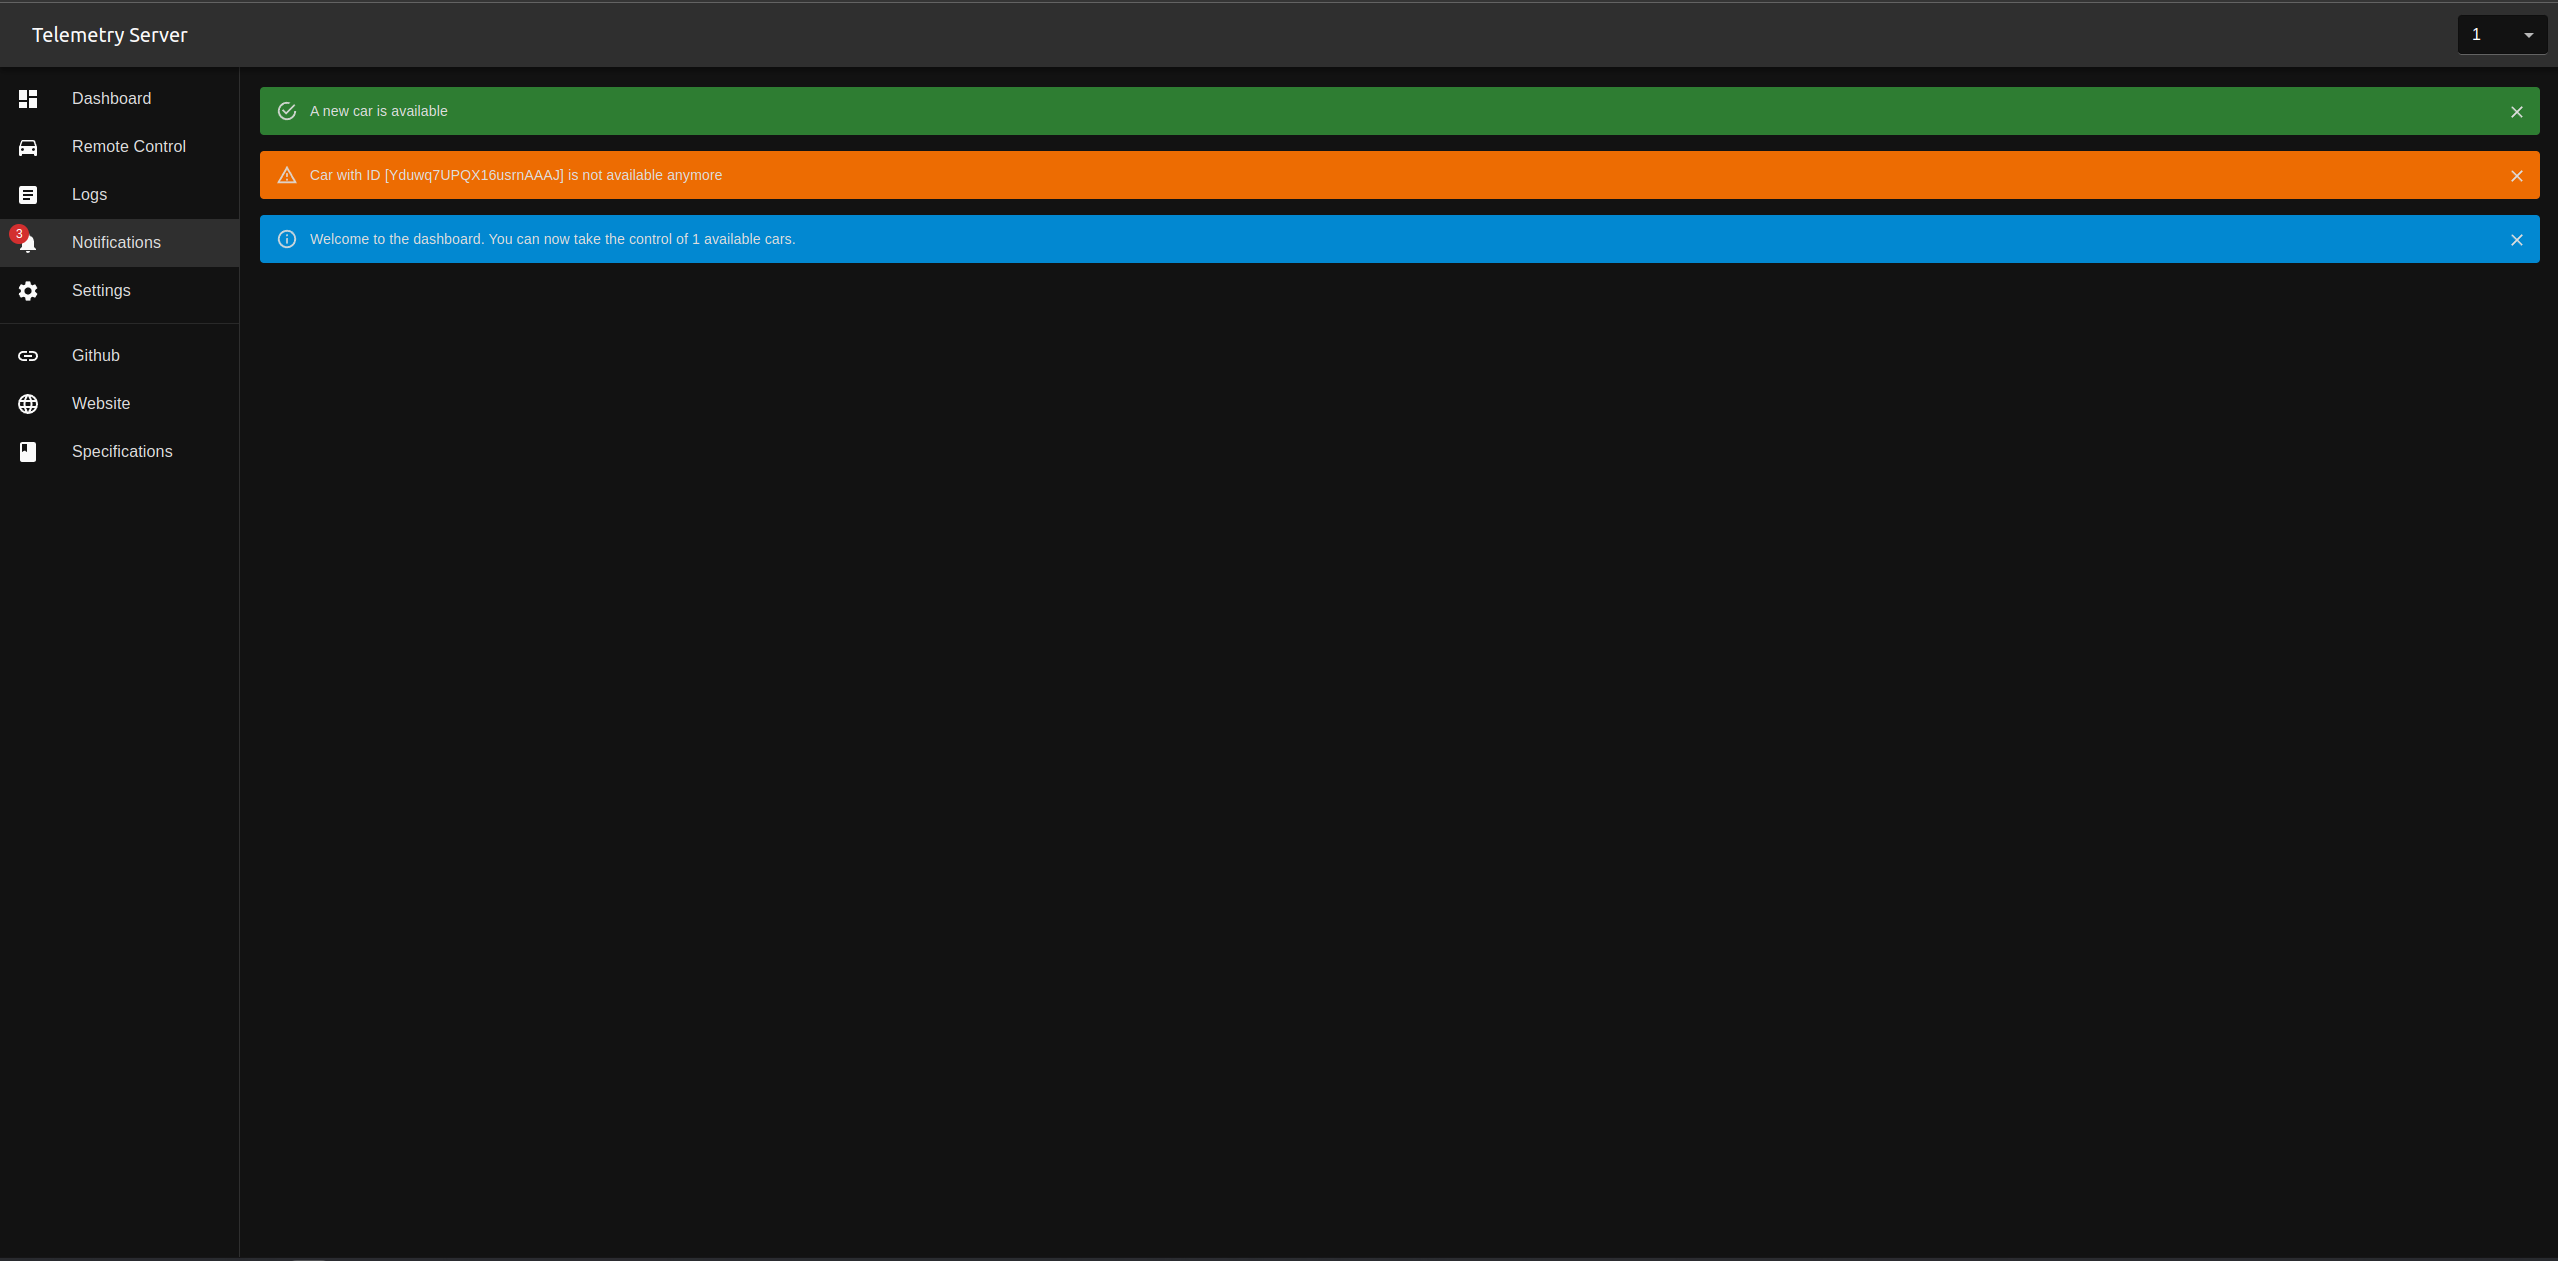
\includegraphics[width=\textwidth]{../../docs/Telem4.png}\\

Here are the “Notifications”. When something happen, We know it. It might be a new Car available for streaming or maybe the server has an important message to transmit for instance when somebody changed the settings of car.\\
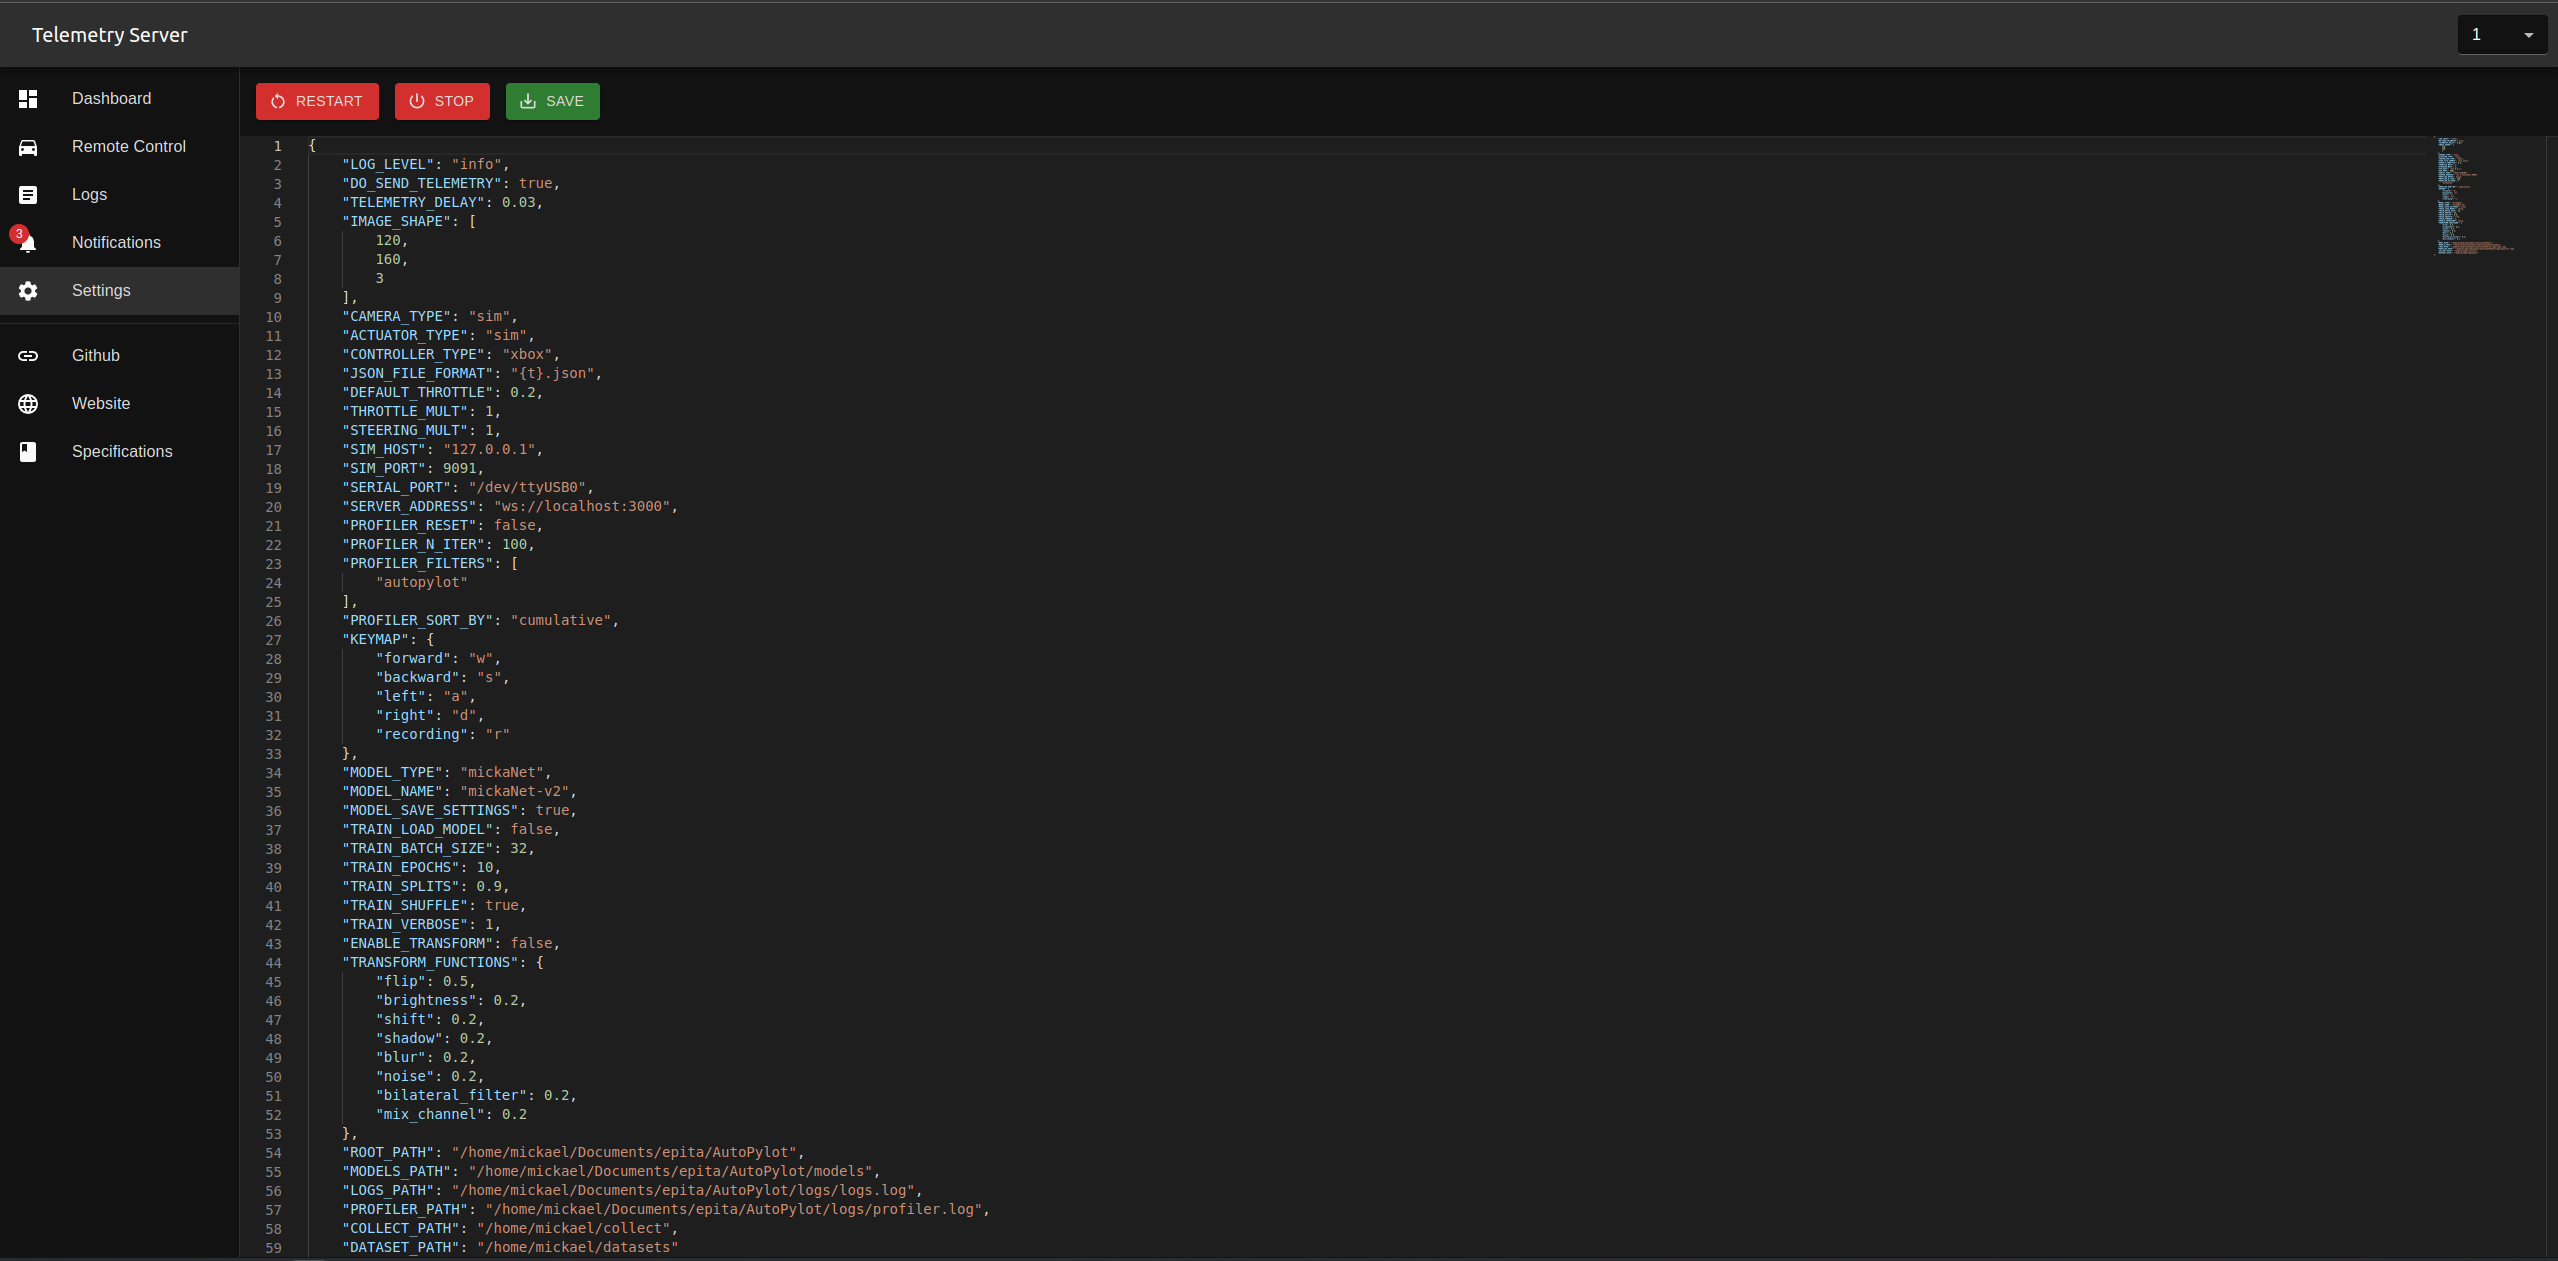
\includegraphics[width=\textwidth]{../../docs/Telem5.png}\\

And eventually here are the “Settings”. This part is crucial. Here we load the “settings.json” from the car. We can update the car’s behaviour, stop or restart with the help of a simple click. This is much better than ssh where we need to stop and start the python script or open vim to changw settings. This features prevent fastidious and repetitive task and provide an excellent testing workflow.\\

In Conclusion this server is the autopylot’s best friend. It’s very easy to use and to install, it can also be accessed on a phone. Every time we use the car, we use this telemetry server. This entire server was developed by hand by our team. We hope to make it even better in the future.\\


\newpage

% Ellerbach
\subsection{Some theory}
Before going further into the DeepLearning part, let's have a quick reminder of what is a Neural Network and a bit of theory behind all of that. \\

\subsubsection{Neural Network}
So, what is a Neural Network? 
A Neural Network or "NN" or "NeuralNet" for short is a black box. The role of a Neural Network is to approximate functions. This can be accomplished with a combination of layers that can be also seen as functions with N parameters and P outputs. Each layer can communicate with the next ones. In most architectures the Neural Network can be visualized as a sequential list of layers, but some are more complex featuring: branches, feedforward and other mystical tricks. \\

This Neural Network by default is only outputting random results, to train it to best approximate our imaginary function, we need one thing: Data! In our case, we need to predict the next action of our car: steering and throttle from an image: the POV of the car. We can also imagine adding other parameters to our black box like the current speed of the car.
During the training process, the prediction (Forward propagation) the model makes along with the expected value are used to correct the weights and inner parameters of every layer (Backward propagation). To have a well-fitted Neural Network, the more the data we have and the best the quality of that data is, the better! \\

Neural Networks are mainly composed of fully connected layers (or Dense layers), those are composed of a given amount of neurons. They receive one or more input signals, do calculation on them and then communicates its output signals to the next layer. The output signal is calculated from the sum of every input multiplied by its weight along with the addition of a bias. The output is then going through an activation function before outputting to the next layers. \\

\centerline{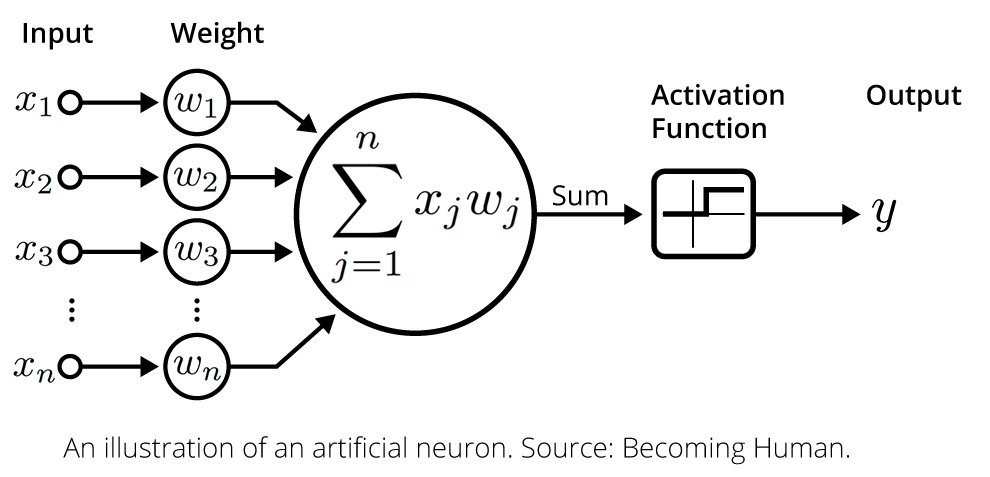
\includegraphics[height=7cm]{../../docs/activation-function.png}}

\newpage

\subsubsection{Convolutional Neural Network}
So now, what is a Convolutional Neural Network?
First, a Convolutional Neural Network or "CNN" is a type of Neural Network! It inherits its name from the kind of layer it has: Convolution layers. \\

What is a Convolution? 
A convolution is an operation that changes a function into something else. It uses kernels or filters to detect features in a signal. In our case, we use two-dimensional convolution. The signal is the image composed of pixels (usually, their values are between 255-0 or 1-0). The main idea behind having convolutions in a Neural Network is to analyze this signal and encode it into a smaller signal. \\
\centerline{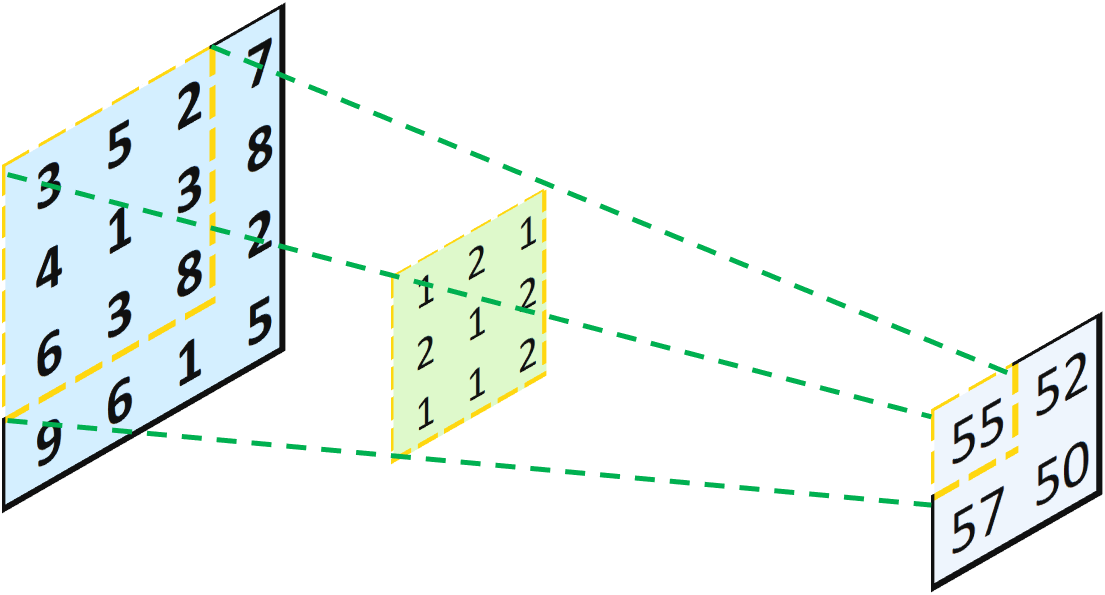
\includegraphics[height=8cm]{../../docs/convolution.png}}

Here you can see the application of a 3x3 convolution kernel on a 4x4 signal, the resulting of the application of this filter is a new signal of size 2x2. The resulting signal is smaller than the input signal, but why is that? Simply because the kernel here is only applied on the valid areas of the input signal, so the outside border of the signal is lost. To prevent that, we can add zero values around the input filters so that the output size matches the input size. \\
\centerline{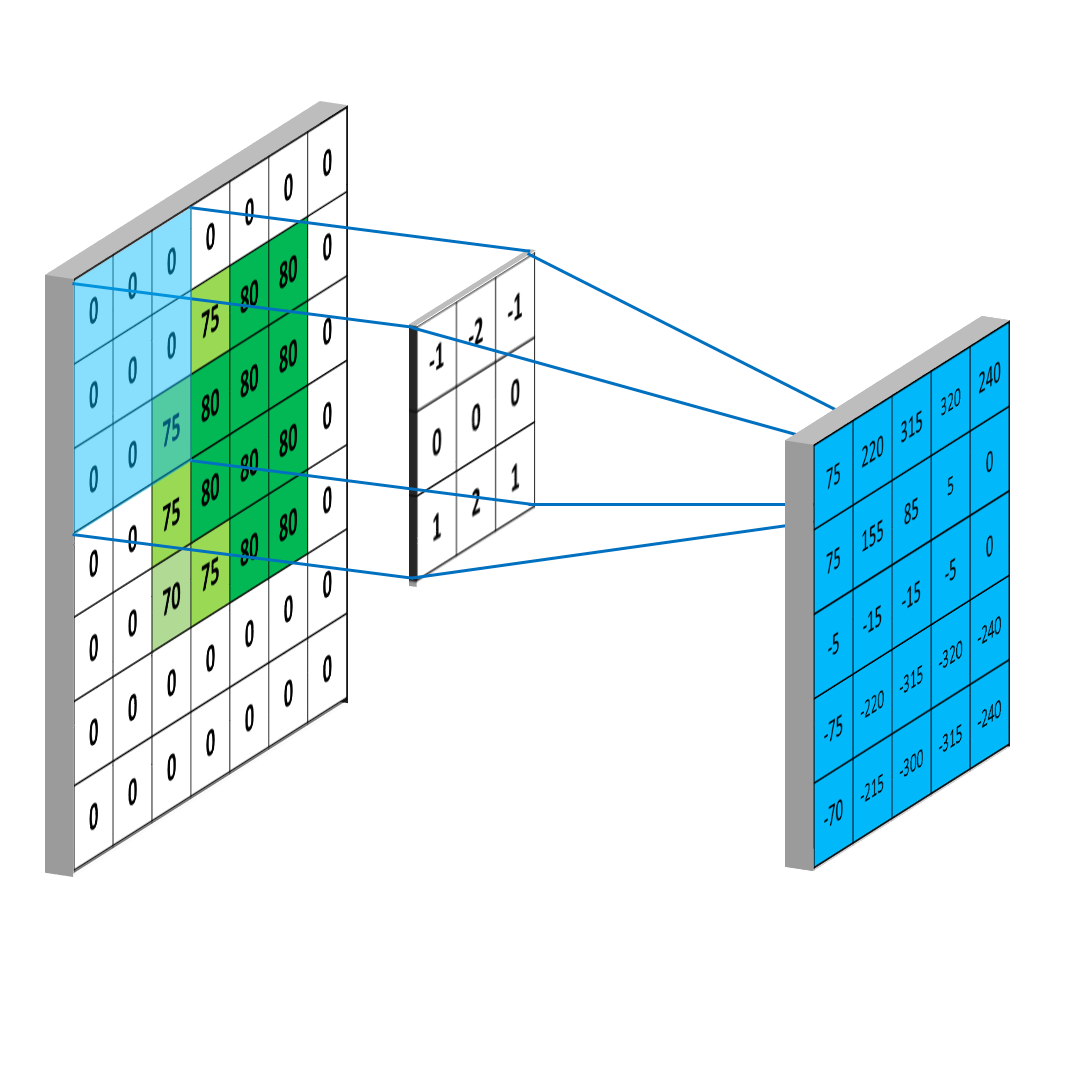
\includegraphics[height=8cm]{../../docs/padding.png}}

\newpage

Now, as said previously, the main idea of having convolutions is to reduce the size of our image, this can be done by introducing strides to our convolution layers. The amount of movement between applications of the kernel of the input signal is referred as the stride. On the above illustrations, we had a stride of 1 meaning at each step, the kernel moved by 1 pixel. On the illustration below, a 3x3 kernel is applied to a 5x5 signal with strides set to 2 without padding. This results in a 2x2 output signal. \\
\centerline{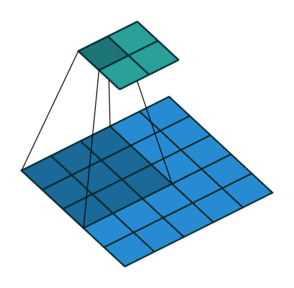
\includegraphics[height=6cm]{../../docs/strides.png}}

Each filter detects simple features from the previous signal but deepest the Convolutional Neural Network is, the more complex the detected features are. Here is an example where we are trying to detect the face of a dog in an image: 
The first convolution layer will detect simple features such as edges on the image. Those can correspond to the shape of the dog as well as the shape of other stuff in the image. The second will have in input the already detected edges, from those edges it could detect sets of edges looking like features coming from a dog: ears, eyes, fur. The third one will from those features detect even more complex features and so on.
After the convolutional layers, we are left with something called the latent space of our image. It is the encoded, simplified form of our image where only the key features are left. From those locally detected features, we can then have a look at the big picture by flattening the 2D signals into a 1D vector to be fed into fully connected layers and then answering the question "Is there a dog in the image?" or "Should we go right or left?". \\

\subsubsection{Activation functions}
In some cases, we want our output signal to meet some requirements, for example, what if we only want outputs between -1 and 1 ? To answer this need, we apply some activation functions to the output of each layer. Here are some of the most popular activation functions. \\
\begin{itemize}

\newpage

\item Rectified Linear unit or "Relu" is the most widely used activation, it cuts off the negative values. It is defined as $ Relu(z) = \max(0, z)$. \\
\centerline{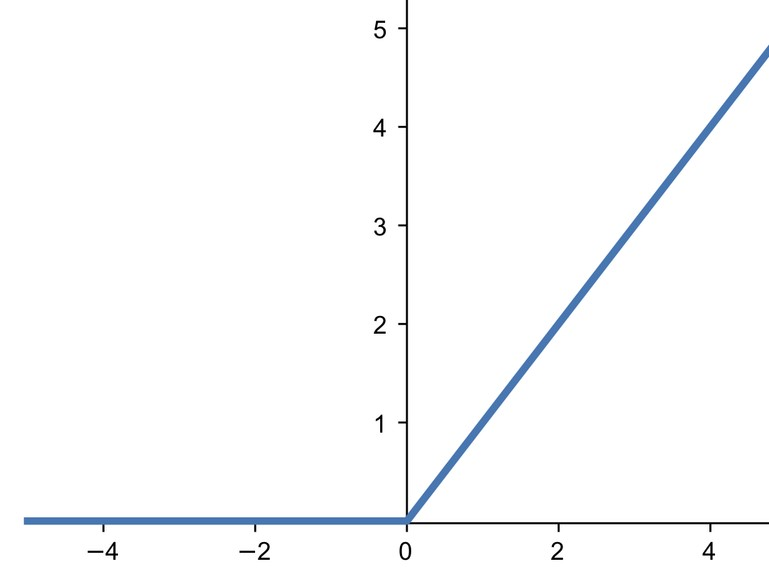
\includegraphics[height=6cm]{../../docs/relu.png}}

\item Sigmoid is another widely used function. It maps every values between 0 and 1. It is defined as $ Sigmoid(z) = \frac{1} {1 + e^{-z}}$ \\
\centerline{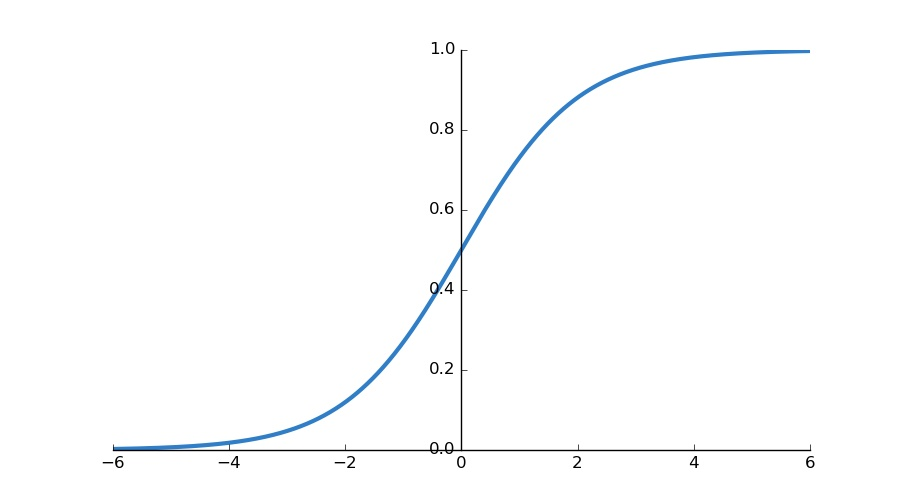
\includegraphics[height=6cm]{../../docs/sigmoid.png}}

\item Tanh, similarly to Sigmoid maps every value between -1 and 1. It is defined as $ Tanh(z) = \frac{1 - e^{-2z}}{1 + e^{-2z}}$ \\
\centerline{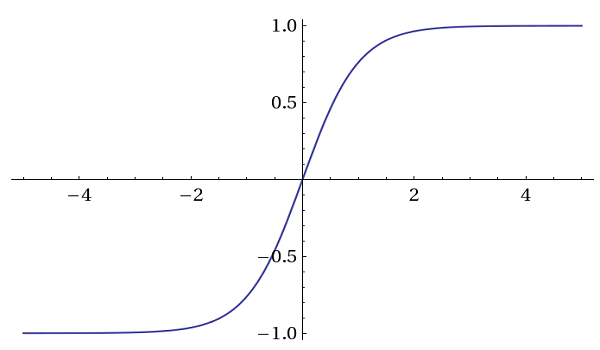
\includegraphics[height=6cm]{../../docs/tanh.png}}

\item Softmax is mainly used for single label classification problems. It is defined as $ Softmax(z_i) = \frac{e^{z_{i}}}{\sum_{j=1}^K e^{z_{j}}} \ \ \ for\ i=1,2,\dots,K$ \\
Here is the plot corresponding to the softmax activation for 2 outputs. \\
\centerline{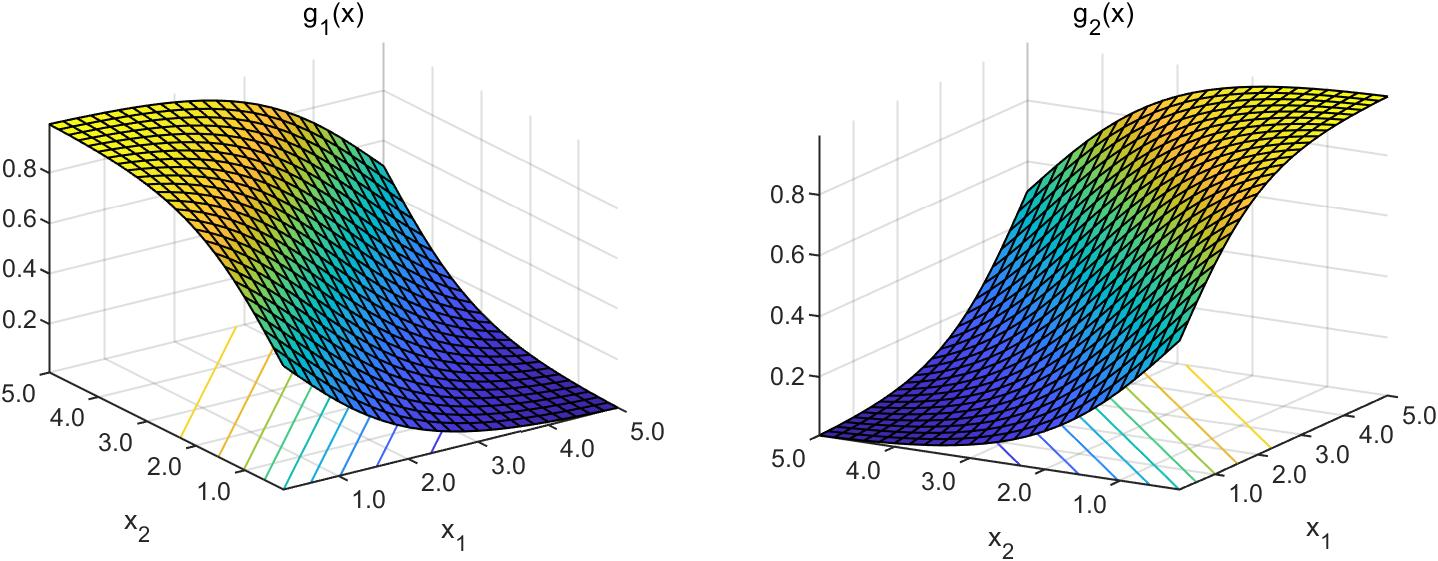
\includegraphics[height=6cm]{../../docs/softmax.png}}

\end{itemize}

% Everyone
\subsection{Model architectures}

So to summarize a bit what was said, a Convolutional Neural Network is a black box that have at least an image as an input and tries to predict something out of this image. As a common trend, the more convolution layers we have, the better our understanding of the image will be. But we have to be careful of how much we should put because we have to keep in mind the performance aspect of our model. In this section, you will see how every member of the team designed their model. The detailed architectures will be at the end of this section. \\

\subsubsection{Maxime Gay}
In order to create my model, I was inspired by the VGG-16 model.

This model was proposed by Karen Simonyan and Andrew Zisserman of the Visual Geometry Group Lab of Oxford University in 2014. It won the ImageNet Large Scale Visual Recognition Challenge (ILSVRC) the same year. The model achieves 92.7\% accuracy in ImageNet. By the way, ImageNet is a gigantic database of more than 14 million of images. At this time, it was a sharp evolution regarding the other models because VGG-16 uses kernels of a smaller size.


Architecture of VGG-16 model :

\centerline{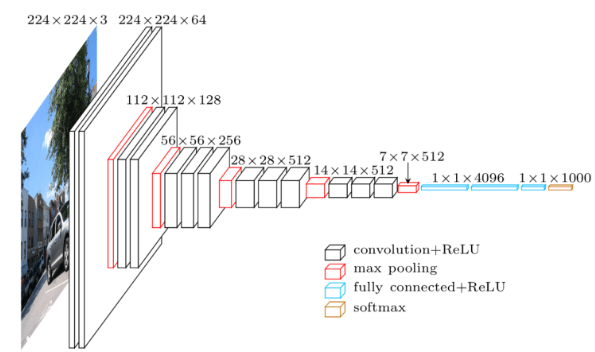
\includegraphics[height=8cm]{../../docs/VGG16.png}}

The problem with this model is that it is slow, and it is even slower in our case because it must work with our car which does not have a lot of resources. Therefore, I decided to change the VGG-16 Model a bit.  

I started by removing some convolutional layers. 

My first convolutional layer has a kernel of 5x5 and not 3x3 to have a filter with a bigger size at the beginning. Furthermore, I start with only four kernels on this first layer to reduce the cost of energy. Then with the other layers, I progressively increased the number of kernels and I reduced the kernel size to 3x3. Moreover, I apply a stride of 2 for the first four layers and a stride of 1 for the last two. In the end, I use two Dense layers with an activation function "relu" like the other layers. Finally, I tested many different optimizers like SGC, Adadelta, Nadam and Ftrl but I decided to use the Adam Optimizer because it gave me the best result. The Adam optimizer involves a combination of two gradient descent methodologies. 

\subsubsection{Mickael Bobovitch}
I Tried different implementation. One that worked pretty well for me is a model inspired by Nvidia. I also tried a model based on the AlexNet Architecture. The common point between architecture is their use on 2D convolution. For instance at the top of the stack, we have 5 layers of 2D convolution, followed by a Flatten Layer and finally by few Dense Layers. Some architetures used MaxPooling to translate images or change the size of the searched object. This technique is great for searching object that can be anywhere on a picture. But form lane recognition this might be not necessary. I am still experimenting a lot. For the next time i will have a more robust architecture. The only challenge for me is to find the best values that can produce a great model.

\subsubsection{Alexandre Girold}
For my part, I decided on making a simple model, capable of steering properly. In order to make this model I spend a lot of time doing some research, and I realized as did my comrades that as of today there is one clear winner in the architecture of a prediction model based on an image. 
It is composed of spatial convolution over images (known as Conv2D) followed by a pooling layer, which is important to avoid overfitting, repeating this a given number of times then followed by a fully connected layer. For these two types of layers, we want to use backpropagation to reduce loss. Finally, the output layer uses functions to give out a probability (I.e: Sigmoid or SoftMax).  

In my model, I tried to reduce the number of parameters to try and make it as light as possible. I also tried to incorporate the capacity for the car to adapt its speed, but as of today, I haven’t been successful. I am sure I will find a solution soon.

\newpage

\subsubsection{Maxime Ellerbach}
When I started to make my model, I thought about: "What could make my model different from the others?" When looking at what my teammates did, it is obvious that the main difference in the model is not in the architecture itself of the model but rather in the data that is fed to it. One other observation is that the less parameters we have in the model, the less sensible it is to overfitting, so the main idea was to have a light model that would also have a rather small latent space. \\

I did see that the combination of [Layer $\rightarrow$ Relu Activation $\rightarrow$ BatchNormalization] worked better with unseen testing images, so I did use this combination for every convolution and Dense layers. \\



\begin{figure}[h]
    \centering
    \subfloat[Model MaximeG]{%
        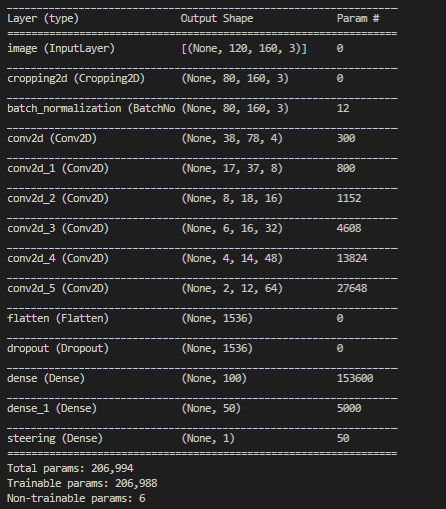
\includegraphics[width=0.49\textwidth]{../../docs/model-maxg.png}%
        \label{fig:b}%
        }%
    \hfill %
    \subfloat[Model MaximeE]{%
        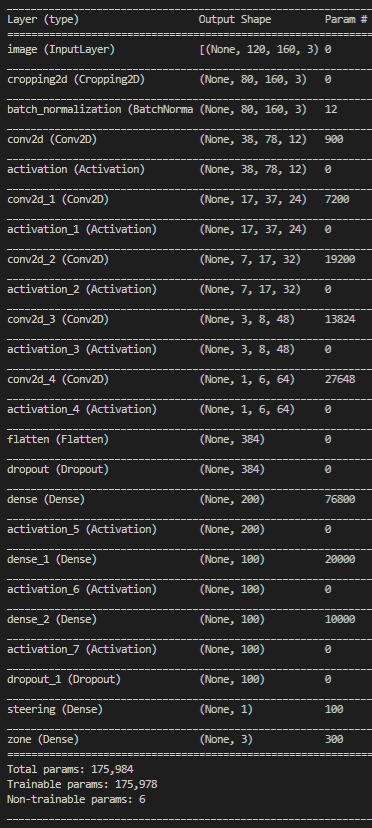
\includegraphics[width=0.49\textwidth]{../../docs/model-maxe.png}%
        \label{fig:a}%
        }%
    \caption{Model Architectures 1/2}
\end{figure}

\newpage

\begin{figure}[h]
    \subfloat[Model MickaelB]{%
        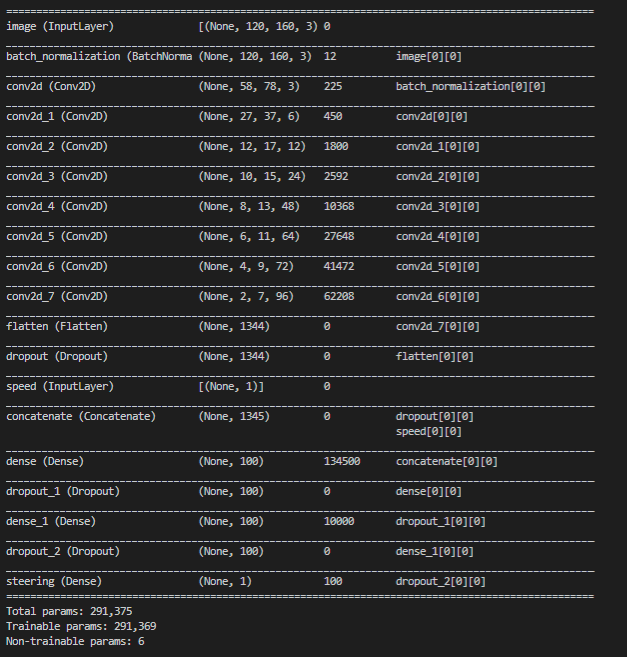
\includegraphics[width=0.49\textwidth]{../../docs/model-micka.png}%
        \label{fig:a}%
        }%
    \hfill %
    \subfloat[Model AlexandreG]{%
        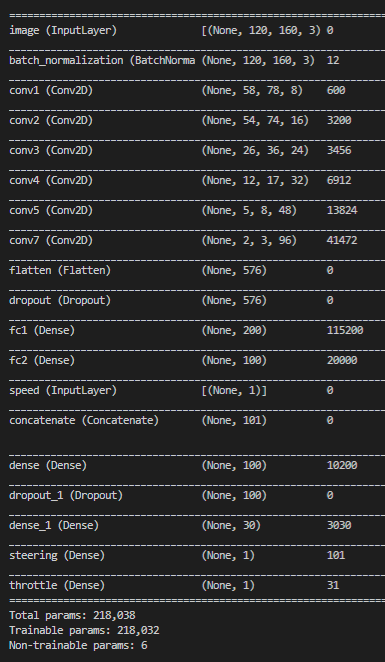
\includegraphics[width=0.49\textwidth]{../../docs/model-sacha.png}%
        \label{fig:b}%
        }%
    \caption{Model Architectures 2/2}
\end{figure}


% Gay
\subsection{Load data during training}
Thanks to the datagenerator file, we can load data to train the model. The class DataGenerator inherits from "Sequence", a tensorflow.keras utils. We give in inputs a list or a list of lists of json paths to train on. To represent those data, we use X to represent the input data and Y the expected outputs. Both are lists of numpy arrays containing the data. Then it returns a tuple containing X and Y.  

How does it work?  

Firstly, we created X and Y which are lists of numpy array. Then we had to pick randomly some paths according to the batch size in order to have more realistic data to train on. Secondly, thanks to the previous function load\_image\_data, we can load the data of the image using a json path

Thirdly, we just have to add the result that we are looking at to the X or to the Y.

\newpage 

% Girold
\subsection{Training Process}

After loading our data, we need to be able to train on those loaded data. The training process is where everything takes place. Indeed, training the data requires the use of all the previous functions. One of these functions is the settings.py. You can see how the function works with the small example below.\\

\centerline{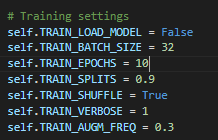
\includegraphics[height=4cm]{../../docs/setting-train.png}} 

This function is the backbone of the training process. It allows us to have a very modular project where everything can be modified from this file only. This allows us to modify our project without deleting a lot of code, making it very modular which was one of our goals from the beginning. For example, we have recently added the telemetry server's restart function, once it was created, we only had to add it to the settings.py and all the other functions would be able to use it.   
This is also useful to change values in real-time. For example, if we want to train our model on more epochs or that our computer can handle bigger batch sizes then we only must change one value and that is it. This goes for all the functions in our project. 

The second import function is of course the train.py function. At first, this function creates all our useful variables (imported from the settings). Then, if the given model does not exist, we create it. For now, this model has not yet been trained.  Then we need to feed the make sure all the variables are correct so that the model can be trained.  To train a model, we need data, in our case images. For this we need to make sure those data exist, and that the path to them is correct.  
We also want to know all the inputs and outputs. This is important as we might want to train not only the steering but also the throttle and speed.  
Finally, we use one important training library. The .fit library from keras. With fit, we are first feeding the training data(X) and training labels(Y) in our case these X and Y come from DataGenerator. We then use Keras to allow our model to train for a given number of epochs and on a given amount of batch sizes. 

% Bobovitch
\subsection{Data Augmentation}
During the learning process we have the possibility to use data augmentation. It’s a technique used to diversify training data and to apply different kind of situations with too much light or not enough. The AI has to consider the road without light effects. Data augmentation is used too add noise on training data. It’s very useful because it forces neurons to find better and more complex features in images. The more features are complex, the less we can experiment overfitting. Which means the AI is more capable to drive in an unknown environment and use complex features to drive better.
\newpage

% Ellerbach
\subsection{Simulator}
Now that we have a trained model, how can we test it ? During the race ! The issue is that every race is separated by a long month of waiting. To avoid waiting so long to test our model, we used a simulator ! \\
The simulator we used is an open source simulator called DonkeySim \\(\href{https://github.com/tawnkramer/sdsandbox/}{https://github.com/tawnkramer/sdsandbox/}) It had been developped using unity. \\ \\

How does it work ?
When a client connects to the simulator, a new car is created, you can choose from a variety of tracks the one you want. You can even create your own tracks ! Then, the server (the simulator) sends telemetry packets to each client (car) connected. Those packets contain data such as an image (simulating a webcam put on the car), some speed data or even odometry data. We can directly feed those data into our previously trained model. The model predicts a steering and throttle value that is being then sent back to the server to apply them on the car. \\

The incorporation of the simulator in our project was made easy by the modularity of it. We only needed to developp the client side: handling the packets, processing the telemetry data, and so on. Basically, the code used to run the real car or a car in the sim is the same, only the source of the data differs. This helped us a lot in the process of developping performant and accurate models prior to deploy them on the real car.

We even recreated the track we are used to race at, this is what the track looks like: \\
\newpage
\centerline{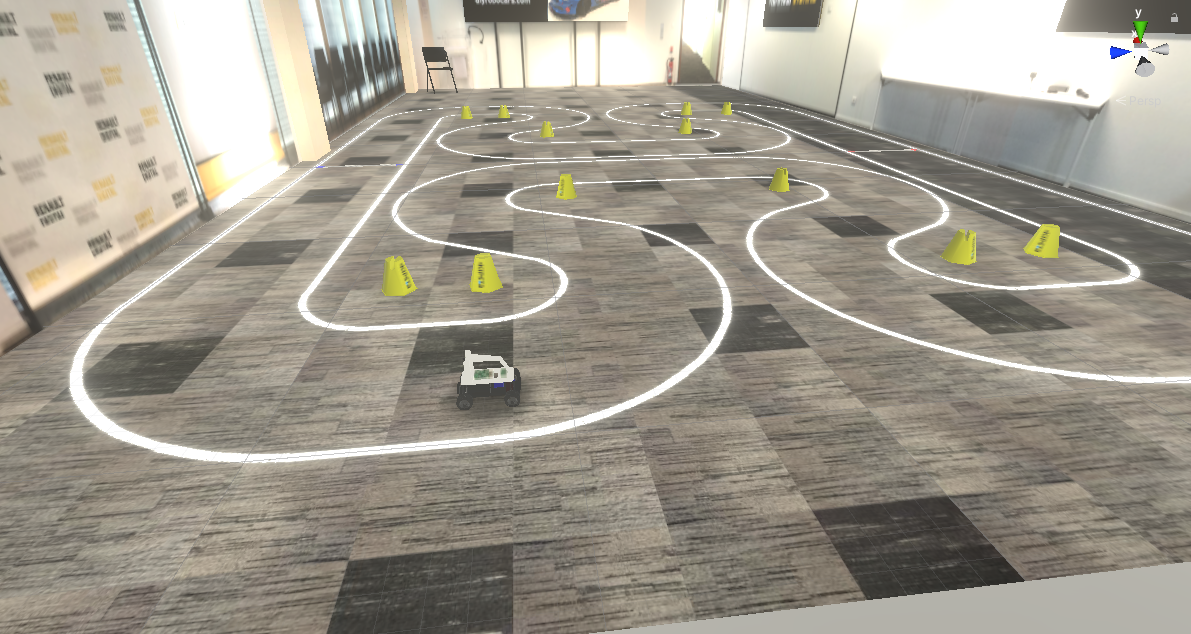
\includegraphics[width=15cm]{../../docs/simulator.png}}
compared to real life: \\
\centerline{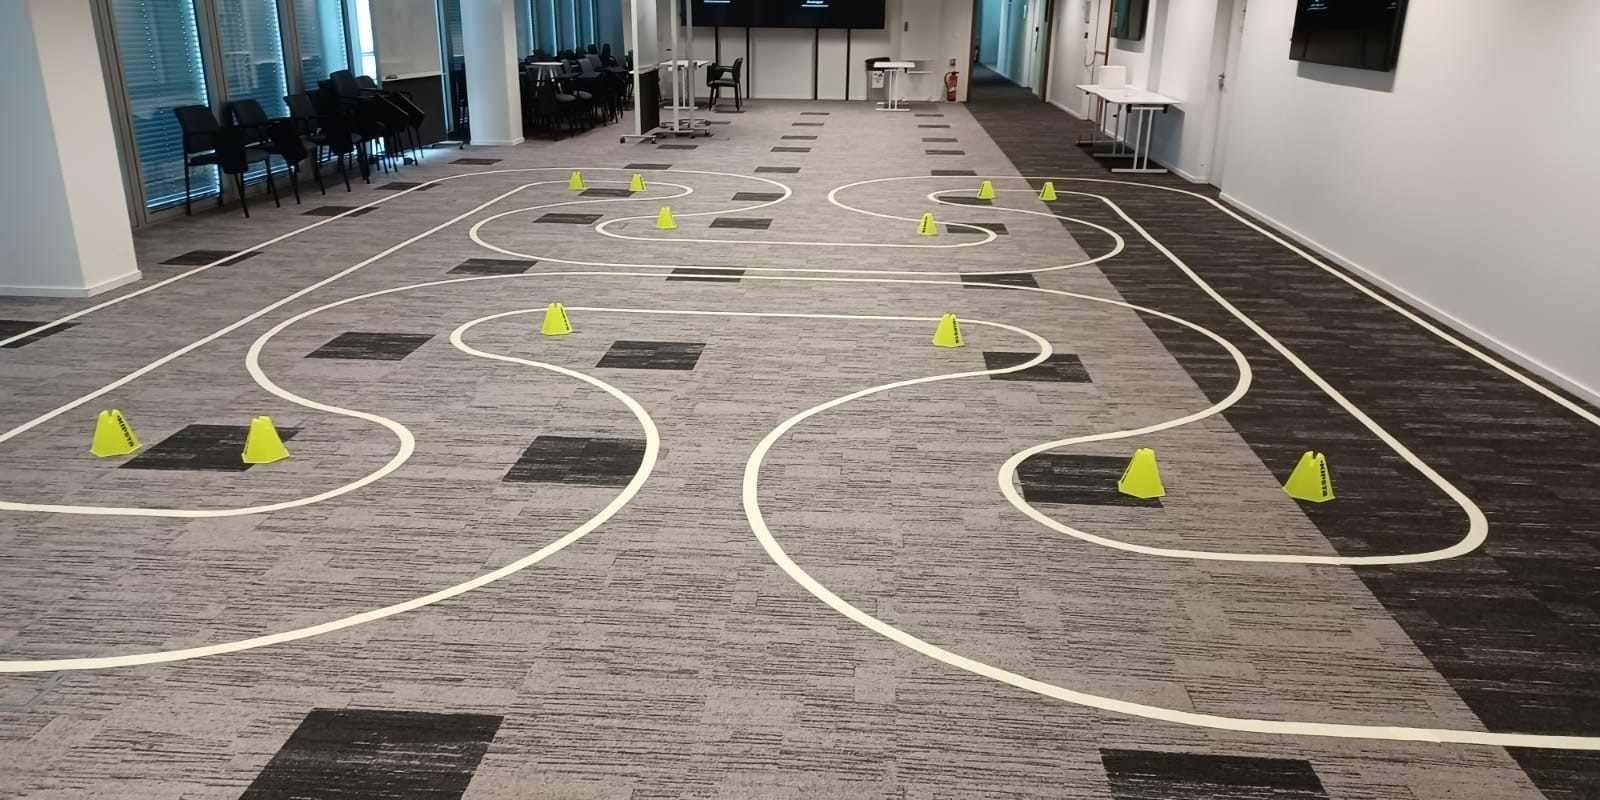
\includegraphics[width=15cm]{../../docs/track-irl.png}}

We created this track using photos took during the races, we took a photo of every wall and a photo of the carpet patterns. Then, we designed the yellow cones we have in real life and imported them into the scene along with the other textures. Then, using the measurements of the track combined with the carpet patterns, we created the floor textures.

Here are the measurements of the track: \\
\centerline{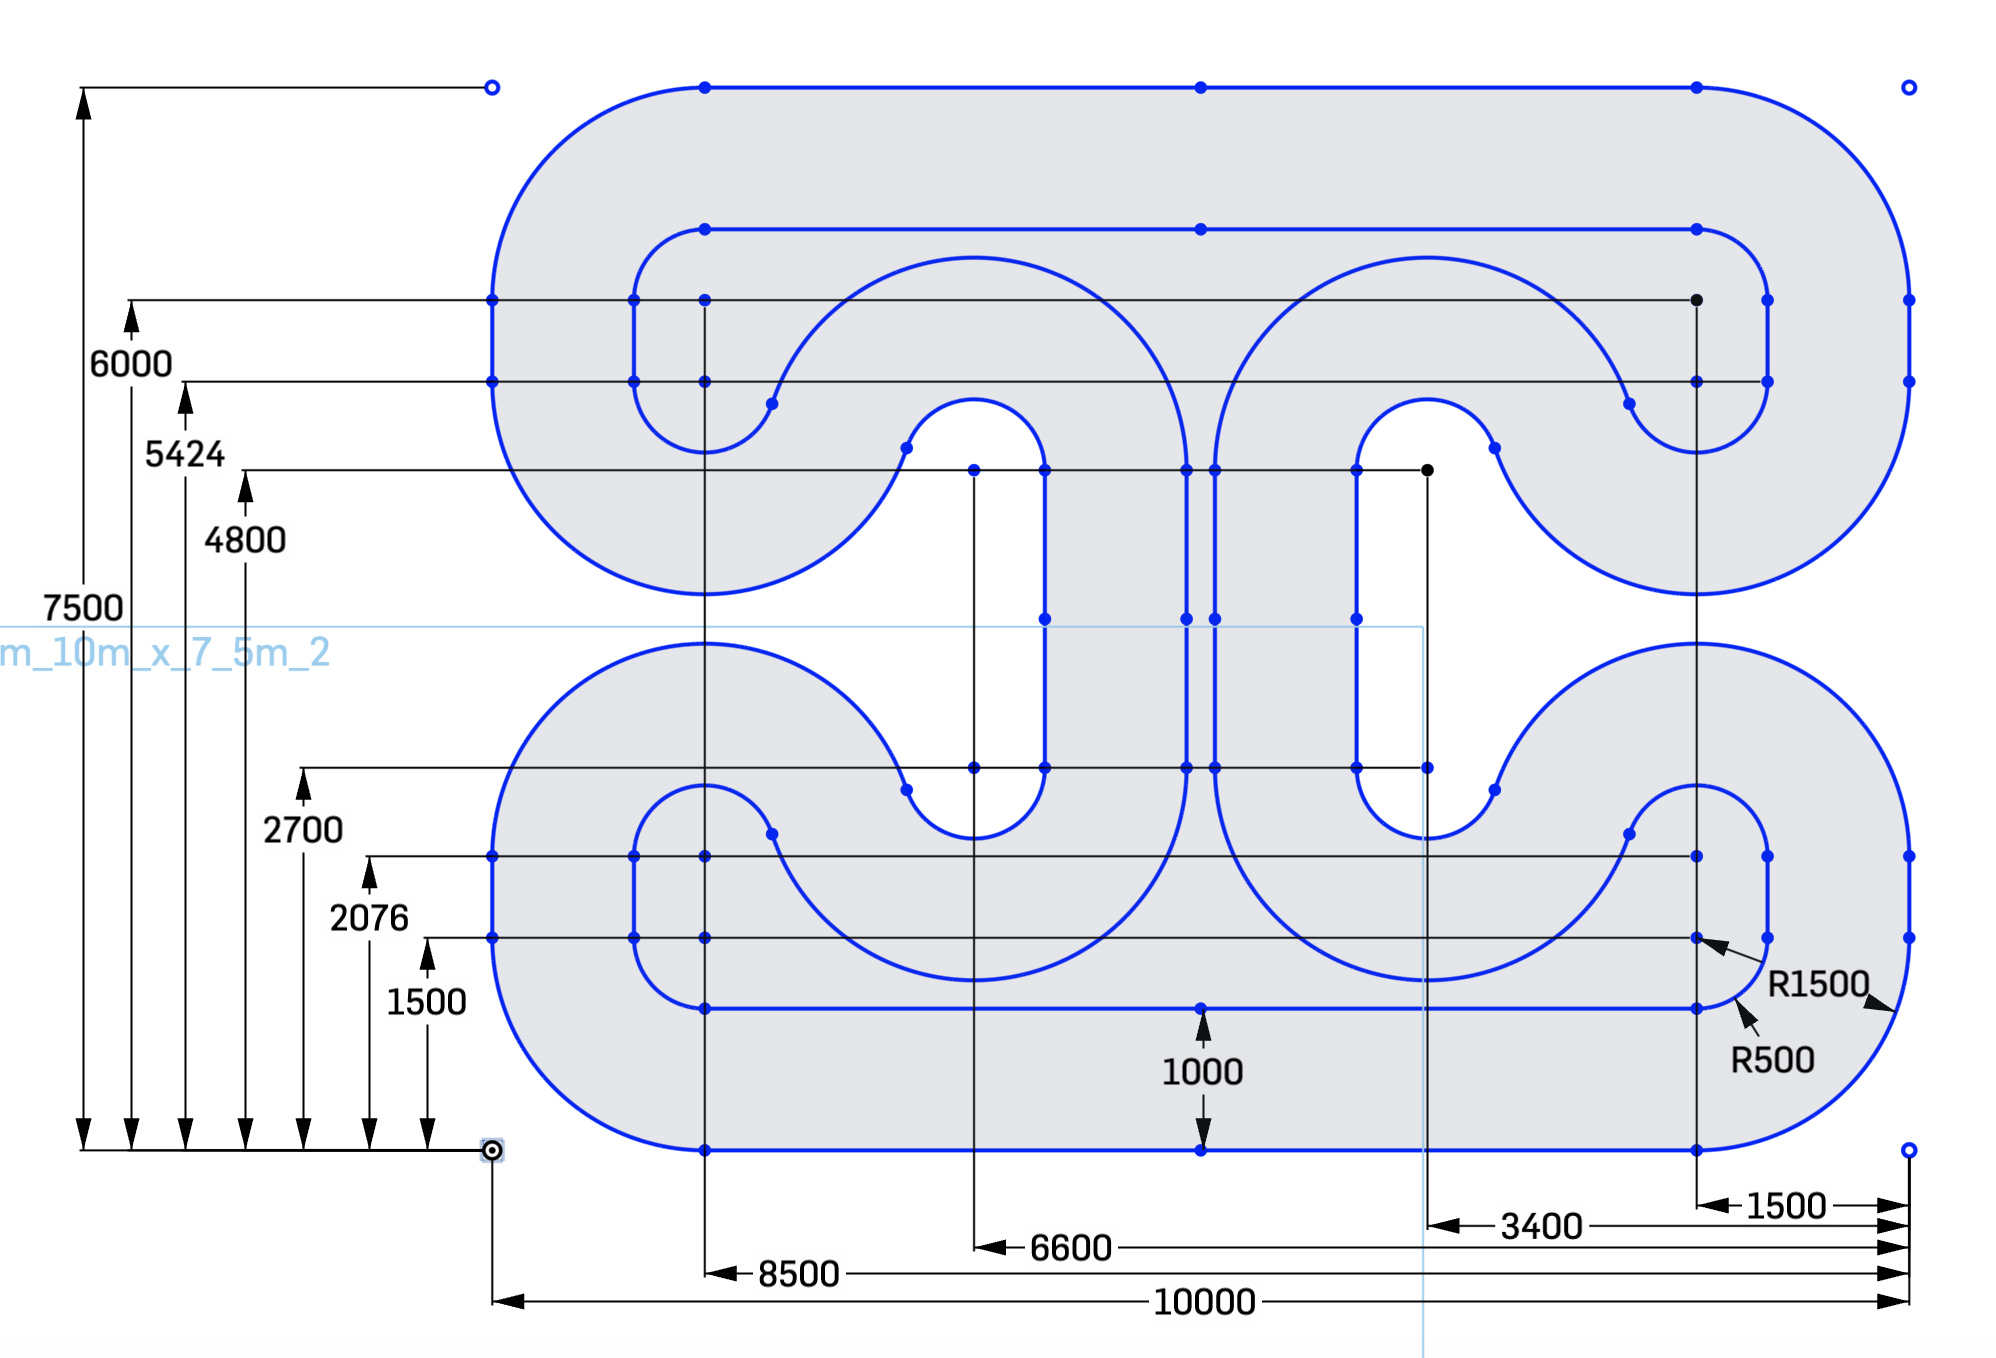
\includegraphics[width=15cm]{../../docs/track-measurements.png}} 

Then, with this scene that looked just like our race environnement, we added all the components required by the simulator to make the client connect and so on. We were then left with a fully working track ! Once our track was finished, we committed a pull request to the simulator's repository and this track made its way into an official simulator release ! We now can train and test our models without having to fire up the real car. We mainly use it to debug our codes and imporve our model architectures.

% Ellerbach
\subsection{Creating some labels}
One of our goal was to handle the throttle using our model to be able to go faster in the straights and slower in the corners. Our first approach was to treat the throttle output just like the steering output by trying to train the model usin gour own throttle inputs. This method did work to some extent. One of the limitation is that our model learns from us, meaning that if we do not respect a precise value in the straights and in the corners, the model would just try to predict an in between values not finding a true correlation between the image and the targetted throttle. \\

So we tried something different: creating our own labels. Theoretically, after collecting a dataset while driving on the center of the track, only by looking at the steering values, we could determine whether we are in a turn, before a turn, or in a straight. This is exactly what we did. We did collect a buch of data by driving multiple laps. Then, we loaded those sorted data and had a look at the mean steering values, it was clear that we could generate some labels from this. So we did continue on this idea, we created a script to analyze those data and determine in which `zone` our car was in. Then we saved those created informations into the corresponding json files. \\

Then, we were required in order to use those new labels to add a new output to our model. This way, we would have as inputs: an image, and as outputs: a steering and 3 neurons corresponding to the following: [are we in a straight, are we in a braking zone, are we in a corner]. The advantage of detecting those zones is that it is really easy to add throttle coefficients to each zones, and those coefficients could be tweaked to offer the best performances. 

% Ellerbach
\subsection{Data Generation tool}
At first, we did use the simulator to gather data, simply by driving around in the simulator just like we would in the real life with the car. By mixing both data collected from the simulator and from our real car, we observed that we acheived better performance, our model did understand better the track. And we wanted to take it a step further and set a goal to automate the gathering of our data.

So we headed to this goal ! The first step was to create a new unity project where we would import our previously created track. Then we asked ourselves, what do we need in order to create data ? A camera, a moving car and a way to tell where the car should go and then save those data.
\subsubsection{Generating images}
For the camera, we used a basic camera from unity where we applied some shaders to modify the field of view of the camera. This is important as the closest the camera looks compared to our real camera, the better our model will be. 
We then measured the position of the camera on our real car as well as the angle to determine where we should put this camera in our data generation tool. \\

\centerline{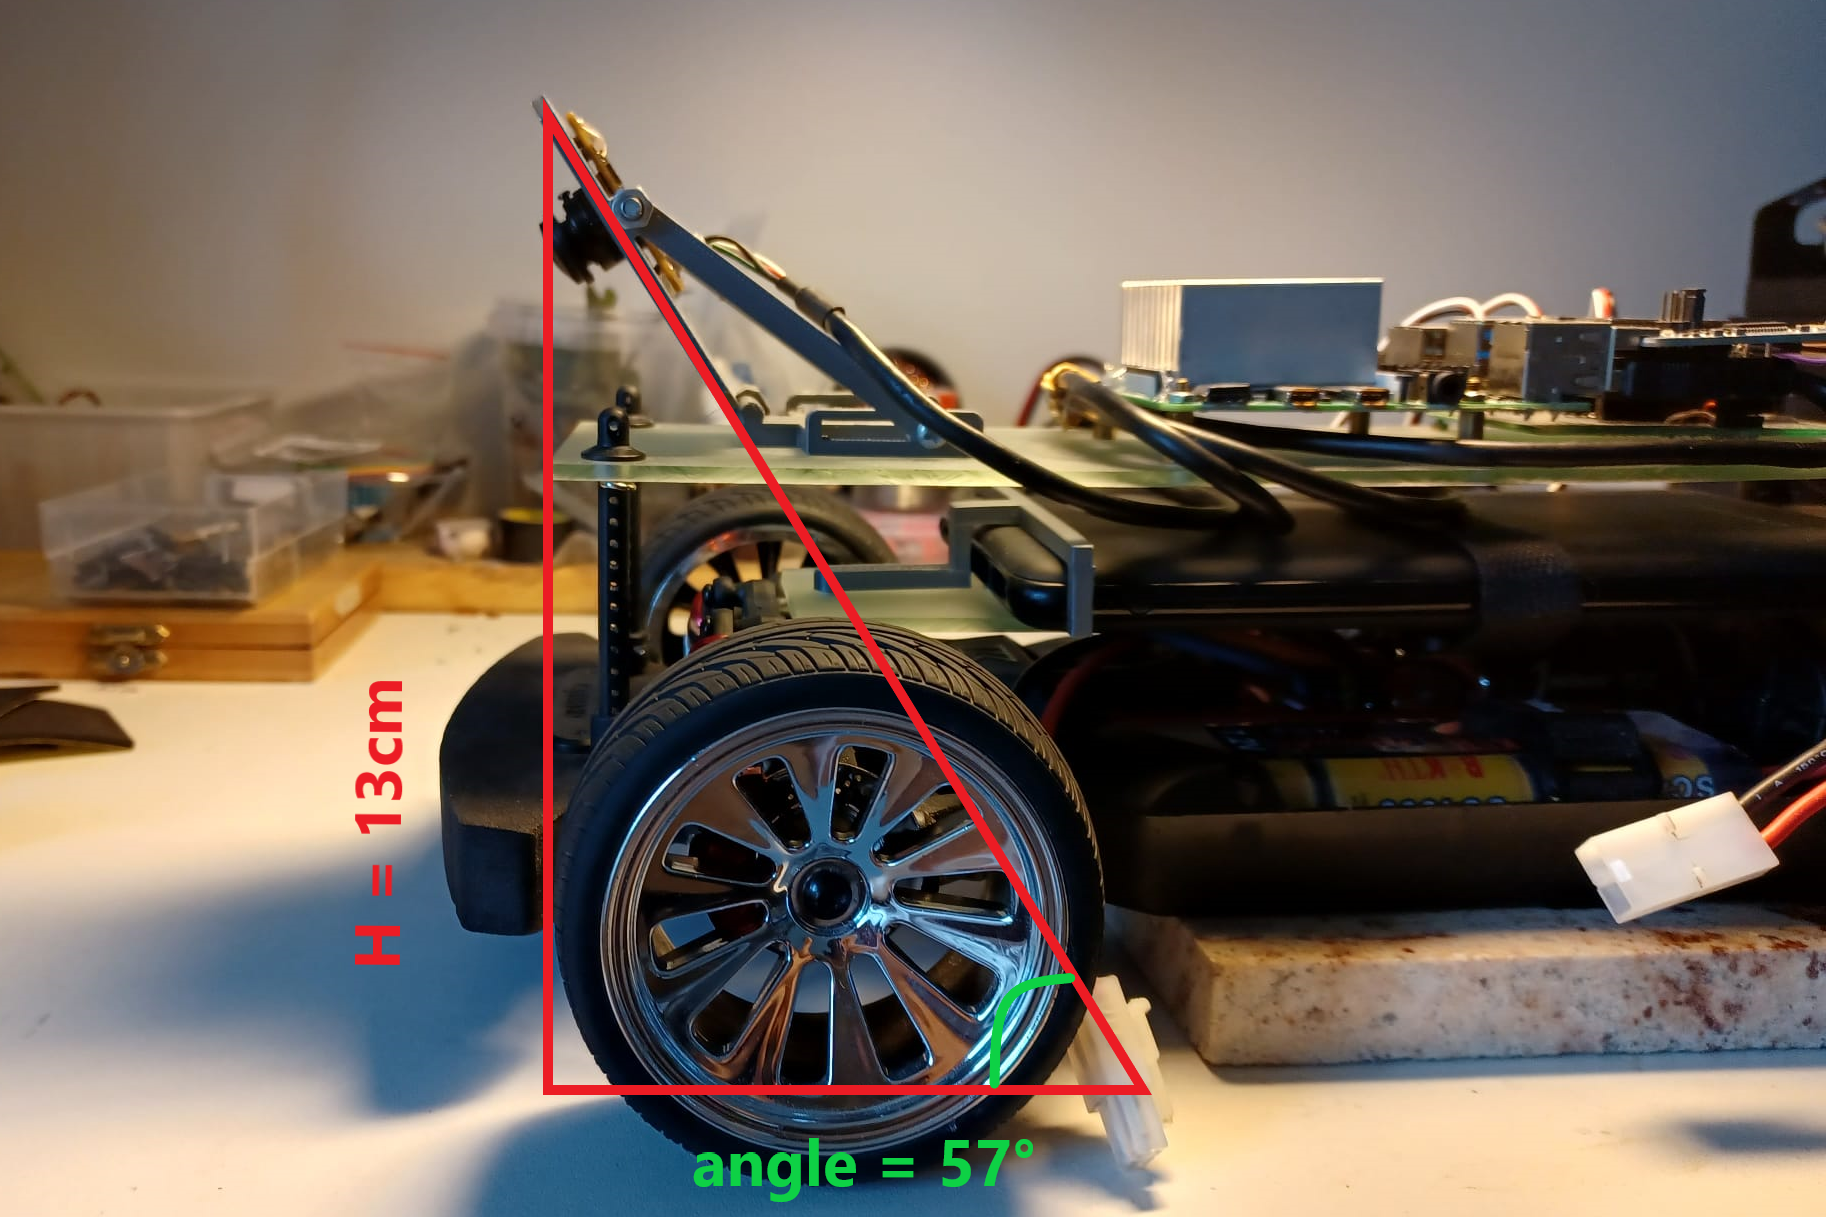
\includegraphics[width=15cm]{../../docs/camera.png}} 
\centerline{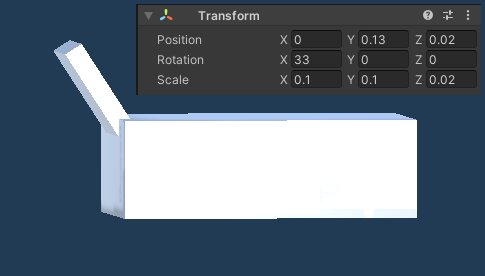
\includegraphics[width=15cm]{../../docs/car-sim.png}} 
Here, the camera won't be seing the car itself, so this design is only indicative for us, a camera object alone would have done the job fine.

\begin{figure}[h]
    \centering
    \subfloat[Real life]{%
        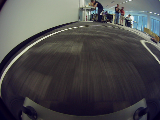
\includegraphics[width=0.49\textwidth]{../../docs/real-camera.png}%
        \label{fig:b}%
        }%
    \hfill %
    \subfloat[Data generation tool]{%
        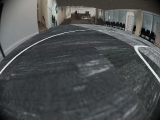
\includegraphics[width=0.49\textwidth]{../../docs/sim-camera.png}%
        \label{fig:a}%
        }%
    \caption{Camera point of view}
\end{figure}
You can see here that the image we are generating is really close to an image that we could get in the real life. You can also note that in the real life we can see a part of the car, whereas in the generated image we do not, that is not a major issue as our model do crops the top and bottom of the image. 

\subsubsection{Generating labels}
Now that we can generate images, we need now a way to generate labels: steering and zones labels. In order to generate them, we will need three splines, one for the ideal trajectory, one for the car trajectory and one for the center of the road. For simplicity, we will consider for the moment the ideal trajectory as being the same as the center of the road. The car trajectory spline is randomized at runtime using the center of the road. This way, by randomizing where the car is located, we can truly generate data that we would not have generated in real life. Indeed, when driving the car on the real circuit, we do not explore cases where the car is off trajectory, and our driving is never perfect, whereas the data generation tool would be able to generate perfect labels for any kind of situation.

Here is the top down view of both center line spline and the randomized car trajectory spline: \\ 
\centerline{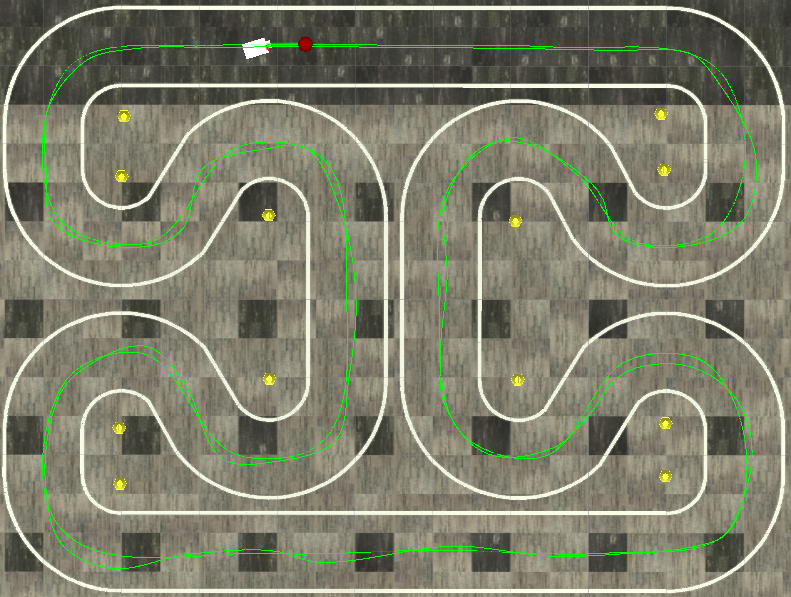
\includegraphics[width=15cm]{../../docs/splines.png}} 

You can distinguish the car on the top of the image along with a red point, this point represents the target point of the car. This point is used to process the steering label. We found a basic policy comparing our orientation and the target orientation along with our lateral position and target lateral position. \\

We can visualize this calculated steering using gizmos: \\ 
\centerline{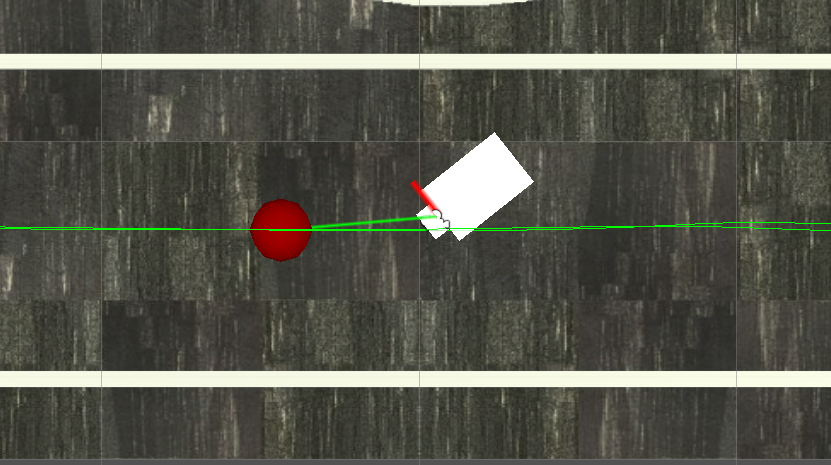
\includegraphics[width=15cm]{../../docs/sim-steering.png}} 

\newpage
Here the red line represents the steering angle. In this particular example, the calculated steering angle is +17,25 degrees and our maximum steering angle is 25 degrees, so the car is turning quite sharply to the right which is coherent with the fact that the car position and angle are quite off. \\

But what about the new `zones` label we previously talked about ? \\

Having at our disposition a spline located at the center of the road, we can establish a map of mean angles by taking small segments on the spline and processing their angle difference, from this map we can process a mean and apply a threshold.
Here is a visualization of those mean angles: \\
\centerline{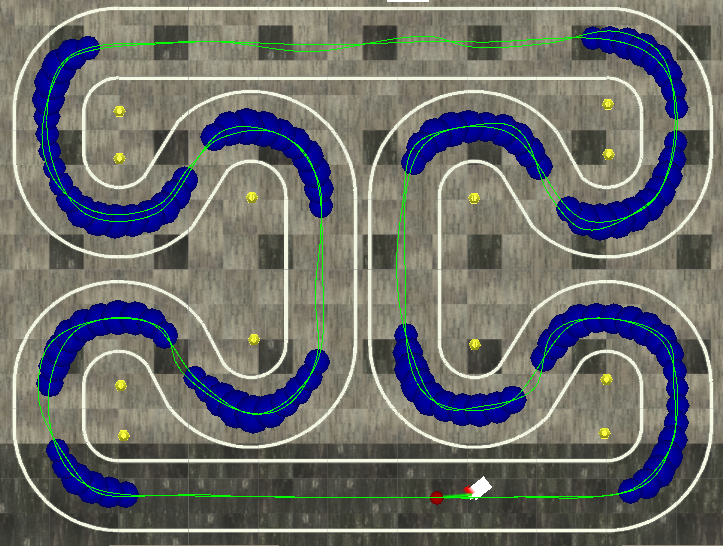
\includegraphics[width=15cm]{../../docs/sim-zones.png}} 

The bigger the blue point is, the bigger the mean is. Using this map, we can go even further, and apply directly our previously developped algorithm for the zones labels. And that's it ! We have our new labels.

\subsubsection{Generating random speeds}
Speed also affects how we drive, so not generating those informations would be a huge mistake as one of the parameters that makes our car fail in real life is the speed. The car struggles when it goes too fast or too slow compared to the speed it was trained at. We can fix that by randomizing the speed in our data generation tool. As you may have noticed, we already use the X and Z axis of our spline, but one axis is left unused: the Y axis (the height). We will use this axis to store our random speeds.

Here is a side view of the car trajectory spline with the height representing the speed of the car: \\
\centerline{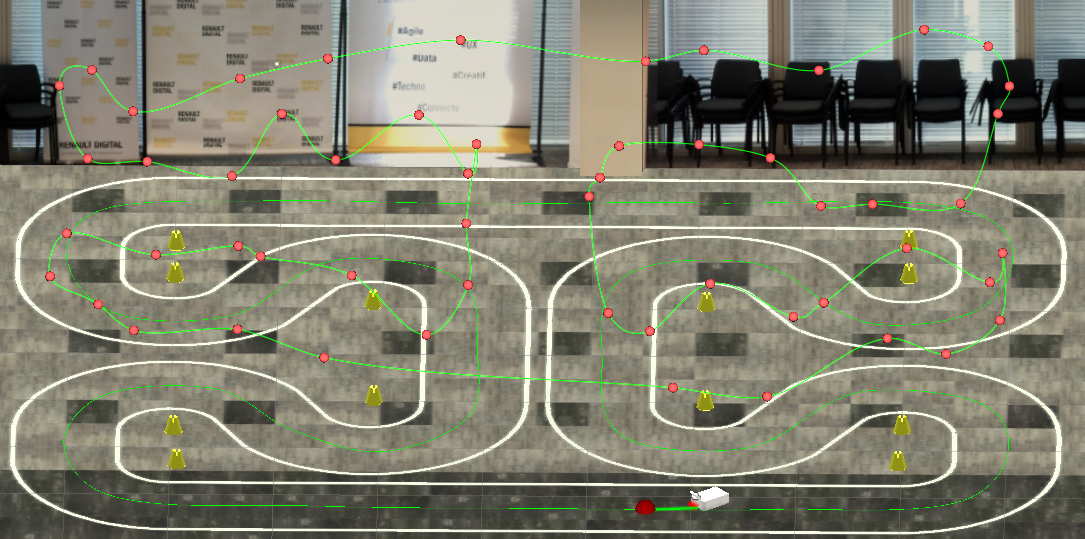
\includegraphics[width=15cm]{../../docs/sim-speed.png}} 

But how will the speed of the car affect the other previously generated labels ? \\

For the steering, the red target point is in fact placed at a given distance in from the car's position, we previously considered the speed as constant, so we can easily now express this distance as a function of the speed. So as the speed varies, the distance to the red target point also varies. A higher speed mean a larger distance to the target point. We can see this as: the faster you go, the further you need to look ahead.

For the zones labels, the speed doens't impact the location of the car so it won't affect those labels. But still it is important to mention that we do use the speed of the car to ensure a minimum speed threshold when in a corner or in a braking zone. The ideal scenario is that we do reach the minimum speed in the braking zone, just before the corner.


\subsubsection{Randomizing the environment}
It is really important for our model to explore different environment to avoid overfitting. If it is presented always the exact same track in the same conditions, it will learn to steer using features that are not linked to the track layout, such as where the chairs are located or even what does the windows look like. We obviouslyt do not want that !
To avoid this behaviour, we randomized this scene. every N seconds, we changed the lightnings, and the objects in the scene. We did create a range of probable lights ranging from blueish to yellowish light. For the props, we did place randomly around the track some chairs and tables. It is quite easy to do this because we do have access to the road center spline from which we can deduce the exact location of the track and thus not place any props on the track. \\

We are now ready to fully use our new tool to generate data !
We can generate up to 200 images per seconds, which is 6 times faster than our regular data gathering speeds.
Here is a sample of a folder of generated data created in a few seconds: \\
\centerline{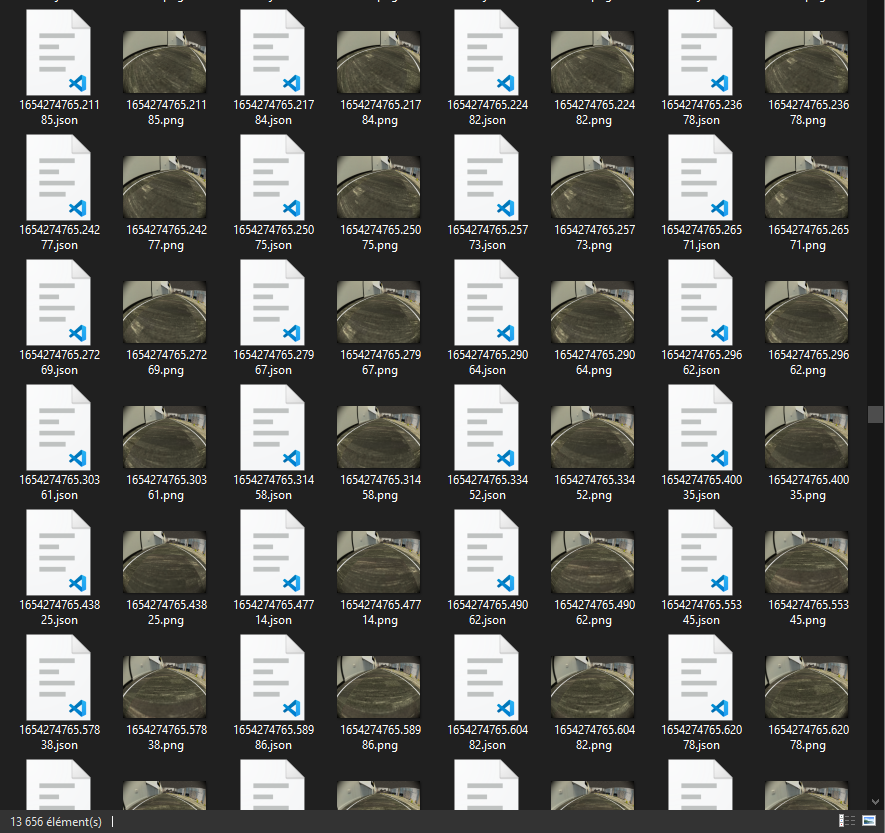
\includegraphics[width=15cm]{../../docs/sim-folder.png}} 

% Ellerbach
\subsection{Overtaking}
Our last optionnal objective was to be able to overtake a car properly. Unfurtunetly, we didn't have the time to do this one. When looking back at what we said we would do, we exceeded our objectives and did extra work on working with unity by creating a digital clone of the track and a data generation tool from scratch. Those turned out to be more useful compared to the overtaking algorithm as the races we do stop once our car catches up with the car ahead.

But we still have this goal in mind and we will try to accomplish it ! To make it work, we have in fact a lot of things already done. We have implemented a data generation tool which we could use to put a 3D object (a car) in front of the camera. We will then need tomodify the functions used to generate the steering values, add a bit of randomization in between, and here we have it !
An other approach would be to add randomly images of cars directly during our training using our data augmentation pipeline. Again, we pretty much did all the work, we only need to had a few functions to take care of this.

\newpage

% Bobovitch
\subsection{Website}
As seen before we already developed a web app for our telemetry server. Also, in parallel we developed a static showcase website (available at \href{https://autonomobile.github.io/}{https://autonomobile.github.io/}). \\

This site is purely static. The mission is to keep it the most professional and simple possible. It is still under construction. We eventually add new content and sections as our progression follows. Our site aims to reflect the efforts and motivation of our team. To deploy the site, We used the excellent quality service offered by Github Pages. \\

We have created our own organization on GitHub, as it enable us to publish the project under our team’s name. Hosting our site in the same place as our code repository allows us to offer a greater visibility to people. Moreover, for the development, it is even easier to manage because all resources are in the same place. \\

In both cases, We used the Next.js framework, a React framework. It allows the creation of web applications and static websites. In terms of stylling, we used UI libraries such as Tailwind CSS and Material UI to increase productivity and produce content that met the high standards of the web in 2022. With Next.js the backend and the frontend part are merged together which help the development process. \\

In this project we aim to learn the best practice regardless of the technology used. As learning remains our main goal.


% Girold
\subsection{Creation of the logo}
\centerline{
\includegraphics[height=8cm]{../../logos/logo-transparent-black.png}}

As we were working on our project, we decided it needed a visual identity that could be easily remembered yet have meaning behind it. With this idea in mind, we brainstormed all together and came up with something new, something we believe is a good compromise of information style and personal touch. After a lot of work, we have come up with the logo printed above. Of course, by now, our visual identity has a different version, each of them answering to a problem we have faced or will face. We have used a variate of tools from simple google research to an extensive use of PhotoShop.\\

But what is the meaning of this piece of craftsmanship?\\

It has a couple of meanings, the first one being the red circle which in our vision represents a track, an unfinished as there is always room for improvement in any project. The second one is more subtle. The second one is the four dots on the top of the circle. These four dots each represent an autonomous vehicle racing on the track. Why four? Because we are a team of four young and hardworking developers. Finally, the most obvious one is the name of our project in the middle of the circle. 

% Girold
\subsection{Realization of t-shirt}
\centerline{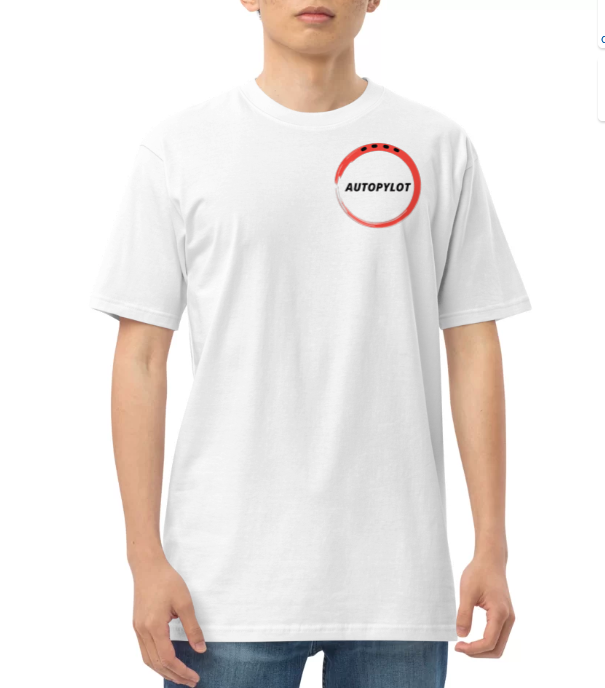
\includegraphics[height=8cm]{../../t-shirts/white_t-shirt.png}}
Yes, we have decided to make t-shirts, why because we want to show how much we are devoted to this project. We honestly want it to be a success and a way to learn essential tools for future projects.\\ 

The t-shirt took a bit of work as we spend a couple of hours deciding on the fabric’s quality and what to put on it. Thankfully we already had a visual design for the front, yes, I am talking about the logo Autopylot.  On the back we have decided the put the name of our team “Autonomobile”, but if a particular form which resembles a wheel. \\ 

To make our purchase we have used a site with a good reputation and pretty good quality products. The name of the website and company is Printful.  We are quite happy with the result and are proud to wear these t-shirts on for any occasion we will have to promote our project. 

\newpage

% sout : 7 / 03 & 25 / 04 & 06 / 06
\section {Planning}
\subsubsection {What is next ?}
The objectives we set ourselves for this presentation were acheived. Our final objective will be to win the race at the Vivatech.

\subsubsection {Races}

\begin{tabular}{|l|c|c|c|c|c|c|}
\hline
Tasks & Race 1 & Race 2 & Race 3 & Race 4 & Race 5 & Race 6  \\ 
\hline
Code controlled motors and servo                & 75\%   & 100\%  &        &        &        &         \\ 
\hline
Drive the car with a controller                 & 25\%   & 100\%   &        &        &        &         \\ 
\hline
Data collection                                 &        & 50\%   & 100\%  &        &        &         \\ 
\hline
Telemetry server                                &        & 25\%   & 100\%  &        &        &         \\ 
\hline
Logging                                         &        & 25\%   & 100\%  &        &        &         \\ 
\hline
Data processing and augmentation                &        &        & 50\%   & 75\%   & 100\%  &         \\ 
\hline
Basic Convolutional neural network              &        &        & 25\%   & 50\%   & 100\%  &         \\ 
\hline
\begin{tabular}[c]{@{}l@{}}Advanced \\models and optional objectives\end{tabular} &        &        &        &        &        & 50\%    \\
\hline
\end{tabular}

\subsection {Presentations}

\begin{tabular}{|l|c|c|c|} 
\hline
Tasks                                                                             & 1st presentation & 2nd Presentation & Final presentation  \\ 
\hline
Code controlled motors and servo                                                  & 100\%              &                &                    \\ 
\hline
Drive the car with a controller                                                   & 100\%              &                &                    \\ 
\hline
Data collection                                                                   & 75\%               & 100\%          &                    \\ 
\hline
Telemetry server                                                                  & 25\%               & 100\%          &                    \\ 
\hline
Logging                                                                           & 25\%               & 100\%          &                    \\ 
\hline
Presentation website                                                              & 100\%              & Update         & Update             \\ 
\hline
Data processing and augmentation                                                  &                    & 75\%           & 100\%              \\ 
\hline
Basic Convolutional neural network                                                &                    & 75\%           & 100\%              \\ 
\hline
\begin{tabular}[c]{@{}l@{}}Advanced \\models and optional objectives\end{tabular} &                    &                & 50\%               \\
\hline
\end{tabular}


\section {Task allocation}

\begin{tabular}{|l|c|c|c|c|} 
\hline
Tasks                        & Mickael B. & Maxime G. & Alexandre G. & Maxime E.  \\ 
\hline
Low level car control        &            &           &              & x          \\ 
\hline
Driving with a controller    &            & x         & x            & x          \\ 
\hline
Dataset handling             &            & x         & x            &            \\ 
\hline
Data processing              & x          & x         & x            & x          \\ 
\hline
Data visualization           &            &           &              & x          \\ 
\hline
Telemetry server             & x          &           &              & x          \\ 
\hline
Logging                      & x          &           &              & x          \\ 
\hline
Presentation website         & x          &           &              &            \\ 
\hline
Convolutional neural network & x          & x         & x            & x          \\ 
\hline
Main control loop            & x          &           &              &            \\
\hline
\end{tabular}

\section {Conclusion}
 To ensure the success of the project, Autonomobile team divided the project in different parts. We first improved the control of the car with controller and we worked on the data processing part allowing us to load and save images and metadata. Secondly, we worked on generating useable data putting them into output and inputs. Moreover, we modified the images making them look different from one another to do the training and the future model not overfit. Thirdly, we all of us made our own models and we held a little competition to determine the best. This created enthusiasm and teamwork. Finally, we have made a presentation website with useful informations and we also made a Telemetry Server with which we can modify settings, see a lot of important informations and use the server on our phones thanks to a QR code. We are more invested than ever. We are even invited at the Vivatech in Paris to race against other participants and we plan to continue this project beyond S2 as we have planned to make our own tracks for future competitions at Epita.

\end{document}

